\section{Results}
\label{sec:results}

The results are grouped chronologically because each hardware decision depends
on the previous audit, but the interpretation follows the three workflows:
Workflow A tests angle-structured QAE integration of \(g\), Workflow B tests
Grover--Rudolph finite-law preparation and direct evaluation of
\(I_p(f)\), and Workflow C explains why some circuits were accepted, repeated,
mitigated, or rejected before further QPU execution.

\subsection{Initial anomaly and diagnosis}

The first \texttt{ibm\_fez} campaign at optimization level 0 revealed a strong
Workflow-A/Workflow-C interaction in \(g_0,k=2\). The observed hardware
probability was
\(\hat{p}=0.597656\), while the expected value is \(p=0.25\). With 2048 shots
this corresponds to approximately 36 binomial standard deviations, and therefore
cannot be treated as shot noise.

The diagnostic script verified three facts:
\begin{itemize}[leftmargin=*]
  \item the logical \(g_0,k=2\) circuit has exact ideal probability 0.25;
  \item the saved transpiled QASM from the failed run also has exact ideal
        probability 0.25;
  \item backend-noise simulation predicted a moderate bias near 0.28, not the
        observed 0.60.
\end{itemize}
The failure was therefore classified as a compilation-sensitive hardware effect,
not a logical circuit or QASM convention error.

\subsection{Accepted hardware circuits}

Table~\ref{tab:accepted-circuits} reports the accepted Workflow-A calibration
circuits after applying the Workflow-C admission and repeat rules.

\begin{table}[h]
\centering
\begin{tabular}{llrrrrrr}
\toprule
Case & \(k\) & Depth & 2q gates & \(p\) & \(\hat{p}\) & Abs. dev. & Status \\
\midrule
\texttt{g0} & 0 & 5 & 0 & 0.250000 & 0.246094 & 0.003906 & pass \\
\texttt{g0} & 2 & 71 & 19 & 0.250000 & 0.297363 & 0.047363 & watch \\
\texttt{g1} & 0 & 18 & 4 & 0.500000 & 0.504395 & 0.004395 & pass \\
\texttt{g1} & 1 & 78 & 18 & 0.500000 & 0.530762 & 0.030762 & pass \\
\texttt{g1} & 2 & 152 & 36 & 0.500000 & 0.511230 & 0.011230 & pass \\
\texttt{g2} & 0 & 43 & 9 & 0.500000 & 0.506836 & 0.006836 & pass \\
\texttt{g2} & 1 & 167 & 43 & 0.500000 & 0.516113 & 0.016113 & pass \\
\texttt{g2} & 2 & 291 & 79 & 0.500000 & 0.504883 & 0.004883 & pass \\
\bottomrule
\end{tabular}
\caption{Accepted Phase 1 hardware circuit results on \texttt{ibm\_fez}.}
\label{tab:accepted-circuits}
\end{table}

The controlled \(g_0\) repeat reduced the \(g_0,k=2\) anomaly from
\(\hat{p}=0.597656\) to \(\hat{p}=0.297363\) by changing from optimization level
0 to optimization level 2. The repeated point remains in the watch region, but
the corresponding MLAE estimate becomes usable.

\subsection{MLAE estimates}

\begin{table}[h]
\centering
\begin{tabular}{llrrr}
\toprule
Case & Schedule & Exact \(a\) & Hardware \(\hat{a}\) & Abs. error \\
\midrule
\texttt{g0} & \(K=\{0,2\}\) & 0.250000 & 0.241051 & 0.008949 \\
\texttt{g1} & \(K=\{0,1,2\}\) & 0.500000 & 0.499093 & 0.000907 \\
\texttt{g2} & \(K=\{0,1,2\}\) & 0.500000 & 0.499512 & 0.000488 \\
\bottomrule
\end{tabular}
\caption{Accepted Phase 1 MLAE estimates.}
\label{tab:mlae-estimates}
\end{table}

The affine and quadratic stress tests are the strongest results of Phase 1.
Both pass through \(k=2\) at optimization level 2, and both produce sub-\(10^{-3}\)
MLAE absolute errors. The \(g_2\) campaign is especially important because it is
the structurally harder case, with higher degree, larger canonical length, and
the deepest accepted circuit.

\subsection{Reproducibility artifacts}

The accepted Phase 1 summary is generated by:
\[
  \texttt{python3 scripts/summarize\_phase1\_results.py}.
\]
The corresponding CSV and JSON artifacts are stored under:
\[
  \texttt{results/hardware/phase1\_summary/}.
\]

\subsection{Phase 1b simulator comparison}

The first Phase 1b statistical simulator belongs to Workflow A. It compares
MLAE, an IQAE-style adaptive
likelihood proxy, canonical grid QAE, Monte Carlo, and quasi-Monte Carlo on the
same \(g_0,g_1,g_2\) calibration family. For the fixed-schedule hardware
candidate, \(K=\{0,1,2\}\), the simulator gives mean absolute errors near
\(10^{-3}\), consistent with the hardware regime observed for \(g_1\) and
\(g_2\).

\begin{table}[h]
\centering
\begin{tabular}{lllrrr}
\toprule
Case & Method & Variant & MAE & RMSE & Queries \\
\midrule
\texttt{g0} & IQAE proxy & steps=3 & 0.000764 & 0.000950 & 30597 \\
\texttt{g0} & MLAE & \(K=\{0,1,2\}\) & 0.001238 & 0.001556 & 18432 \\
\texttt{g1} & IQAE proxy & steps=3 & 0.000634 & 0.000802 & 38912 \\
\texttt{g1} & MLAE & \(K=\{0,1,2\}\) & 0.001511 & 0.001931 & 18432 \\
\texttt{g2} & IQAE proxy & steps=3 & 0.000748 & 0.000935 & 38912 \\
\texttt{g2} & MLAE & \(K=\{0,1,2\}\) & 0.001459 & 0.001815 & 18432 \\
\bottomrule
\end{tabular}
\caption{Phase 1b simulator comparison between MLAE and an IQAE-style adaptive
likelihood proxy. Query counts are oracle-query proxies under the ideal
binomial model.}
\label{tab:phase1b-simulator}
\end{table}

The adaptive proxy improves ideal statistical error but uses a larger
oracle-query budget. Canonical QAE and MC/QMC are not decisive on this small
calibration family: the amplitudes \(a=0.5\) and the four-point grid create
exact or near-exact degeneracies for several variants. The next simulator
comparison should therefore include non-special amplitudes or larger structured
Grover--Rudolph instances.

The non-degenerate Phase 1b extensions confirm this conclusion. Synthetic
amplitudes \(a=0.17,0.33,0.61\) and larger midpoint-grid functions remove the
most obvious special-amplitude degeneracies. Representative results are shown in
Table~\ref{tab:phase1b-nondegenerate}.

\begin{table}[h]
\centering
\begin{tabular}{lllrr}
\toprule
Case & Method & Variant & MAE & Queries \\
\midrule
\texttt{a17} & IQAE proxy & steps=3 & 0.000553 & 38912 \\
\texttt{a17} & MLAE & \(K=\{0,1,2\}\) & 0.001067 & 18432 \\
\texttt{a33} & IQAE proxy & steps=3 & 0.000692 & 38912 \\
\texttt{a33} & MLAE & \(K=\{0,1,2\}\) & 0.001357 & 18432 \\
\texttt{a61} & IQAE proxy & steps=3 & 0.000703 & 36823 \\
\texttt{a61} & MLAE & \(K=\{0,1,2\}\) & 0.001446 & 18432 \\
\texttt{gr\_affine\_n4} & IQAE proxy & steps=3 & 0.000867 & 33710 \\
\texttt{gr\_affine\_n4} & MLAE & \(K=\{0,1,2\}\) & 0.001443 & 18432 \\
\texttt{gr\_beta\_bump\_n4} & IQAE proxy & steps=3 & 0.000512 & 38359 \\
\texttt{gr\_beta\_bump\_n4} & MLAE & \(K=\{0,1,2\}\) & 0.001035 & 18432 \\
\bottomrule
\end{tabular}
\caption{Phase 1b non-degenerate simulator extensions. IQAE-style adaptation
improves ideal statistical error but uses a substantially larger oracle-query
budget than fixed-schedule MLAE.}
\label{tab:phase1b-nondegenerate}
\end{table}

\subsection{Phase 0-GR audit for larger state preparation}

The first larger Grover--Rudolph audit validates the state loader before any QAE
amplification is attempted. Exact statevector checks give total variation
distance at numerical roundoff level, confirming that the dyadic probability
tree and uniformly controlled \(R_y\) implementation prepare the intended
probability law. The backend-aware audit on \texttt{ibm\_fez} then gives the
cost and noisy-distribution estimates in Table~\ref{tab:phase0-gr-audit}.

\begin{table}[h]
\centering
\begin{tabular}{lrrrrr}
\toprule
Case & Qubits & Grid & Depth & 2q gates & Noisy TVD \\
\midrule
\texttt{gr\_sin2\_half\_n3} & 3 & 8 & 36 & 7 & 0.0241 \\
\texttt{gr\_sin2\_n3} & 3 & 8 & 31 & 7 & 0.0200 \\
\texttt{gr\_affine\_n4} & 4 & 16 & 76 & 16 & 0.0281 \\
\texttt{gr\_beta\_bump\_n4} & 4 & 16 & 70 & 16 & 0.0320 \\
\bottomrule
\end{tabular}
\caption{Phase 0-GR backend-aware audit on \texttt{ibm\_fez}. All exact
statevector total variation distances are below \(10^{-15}\); the table reports
the noisy Aer readout extracted from the backend model.}
\label{tab:phase0-gr-audit}
\end{table}

All four circuits pass the configured depth and two-qubit thresholds. The first
hardware distribution campaign therefore selects
\texttt{gr\_sin2\_n3}, \texttt{gr\_sin2\_half\_n3}, and
\texttt{gr\_affine\_n4}. The decision is deliberately conservative: it tests
two low-cost eight-point distributions and one sixteen-point non-symmetric
distribution before adding QAE amplification.

\subsection{First Grover--Rudolph distribution hardware readout}

The first distribution-measurement campaign was run on \texttt{ibm\_fez} with
2048 shots per circuit. It measures the prepared distribution directly and does
not include QAE amplification. The results are summarized in
Table~\ref{tab:phase3-gr-distribution-results}.

\begin{table}[h]
\centering
\begin{tabular}{lrrrrr}
\toprule
Case & Qubits & Depth & 2q gates & Phase 0 noisy TVD & Hardware TVD \\
\midrule
\texttt{gr\_sin2\_half\_n3} & 3 & 36 & 7 & 0.0241 & 0.0216 \\
\texttt{gr\_sin2\_n3} & 3 & 31 & 7 & 0.0200 & 0.0313 \\
\texttt{gr\_affine\_n4} & 4 & 76 & 16 & 0.0281 & 0.0479 \\
\bottomrule
\end{tabular}
\caption{First hardware measurement of larger Grover--Rudolph prepared
distributions on \texttt{ibm\_fez}. TVD denotes total variation distance between
the measured distribution and the target dyadic probability law.}
\label{tab:phase3-gr-distribution-results}
\end{table}

The two eight-point circuits are stable at the few-percent TVD level. The
sixteen-point affine circuit remains viable but shows the expected increase in
noise sensitivity, with measured TVD 0.0479 versus a noisy-simulation estimate
0.0281. This motivates a second microcampaign focused only on
\texttt{gr\_affine\_n4}, preferably with light Runtime mitigation and no QAE
amplification, to distinguish sampling variation from a systematic
state-preparation bias.

The focused repeat used 4096 shots with dynamical decoupling and gate/measurement
twirling. It reduced the sixteen-point affine TVD from 0.0479 to 0.0341, and
the maximum per-cell deviation from 0.0235 to 0.0086. This result is close to
the Phase 0-GR noisy estimate and supports using the same Runtime options for
the first amplified test.

\begin{table}[h]
\centering
\begin{tabular}{lrrrr}
\toprule
Run & Shots & Runtime mitigation & TVD & Max. dev. \\
\midrule
First \texttt{gr\_affine\_n4} readout & 2048 & no & 0.0479 & 0.0235 \\
Focused repeat & 4096 & DD + twirling & 0.0341 & 0.0086 \\
\bottomrule
\end{tabular}
\caption{Focused repeat of the first sixteen-point Grover--Rudolph distribution
on \texttt{ibm\_fez}.}
\label{tab:gr-affine-repeat}
\end{table}

\subsection{Mitigated distribution suite}

After the amplified \texttt{gr\_affine\_n4} diagnosis showed that the first
Grover iterate is the fragile block, a second distribution-only suite was run
with the same Runtime mitigation used in the affine repeat. This suite has two
roles: it checks whether mitigation is harmless on the already stable
eight-point cases, and it gives the first hardware readout of the deferred
localized sixteen-point profile \texttt{gr\_beta\_bump\_n4}.

\begin{table}[h]
\centering
\begin{tabular}{lrrrrrr}
\toprule
Case & Shots & Depth & 2q & Raw TVD & Mit. TVD & Mit. max dev. \\
\midrule
\texttt{gr\_sin2\_half\_n3} & 4096 & 33 & 7 & 0.0216 & 0.0208 & 0.0100 \\
\texttt{gr\_sin2\_n3} & 4096 & 31 & 7 & 0.0313 & 0.0368 & 0.0200 \\
\texttt{gr\_beta\_bump\_n4} & 4096 & 68 & 16 & -- & 0.0456 & 0.0241 \\
\bottomrule
\end{tabular}
\caption{Phase 5 mitigated Grover--Rudolph distribution suite on
\texttt{ibm\_fez}. ``Mit.'' denotes the run with dynamical decoupling and
twirling. The raw TVD column refers to the first unmitigated distribution
campaign when available.}
\label{tab:phase5-gr-distribution-suite}
\end{table}

The result is deliberately interpreted as mixed evidence. Mitigation is useful
for the sixteen-point affine distribution and neutral for
\texttt{gr\_sin2\_half\_n3}, but it worsens \texttt{gr\_sin2\_n3} from TVD
0.0313 to 0.0368. Therefore DD and twirling should not be treated as automatic
defaults for every short distribution circuit. They are useful experimental
variables that must be reported case by case.

The first \texttt{gr\_beta\_bump\_n4} hardware run is viable but close to the
current risk boundary: TVD is 0.0456 and the largest single-cell deviation is
0.0241. Direct quantities of interest remain informative but functional-dependent. For
\texttt{gr\_beta\_bump\_n4}, the measured mean \(x\) is accurate within
0.0012, while \(\sin(\pi x)\) has error 0.0177 and the second moment has error
0.0055. This confirms that localized profiles should be benchmarked through
quantity-of-interest error, not only global distribution distance.

A follow-up credit-free audit was then run for the exact localized Phase 5
profile \(F(x)=x(1-x)^4\). This distinction matters because the earlier
Phase 0-GR beta-like profile used different beta parameters. The audit correctly
predicted that the executed candidate was risky: opt-2, seed 12345 gave noisy
TVD 0.0439, close to the measured hardware TVD 0.0456. It suggested opt-3,
seed 45678 as a better candidate, with the same 16 two-qubit gates and predicted
noisy TVD 0.0217. This candidate was submitted as a one-circuit focused repeat.

\begin{table}[h]
\centering
\begin{tabular}{lrrrr}
\toprule
Run & Depth & 2q & TVD & Max. dev. \\
\midrule
Phase 5 opt-2, seed 12345 & 68 & 16 & 0.0456 & 0.0241 \\
Phase 5b opt-3, seed 45678 & 70 & 16 & 0.0502 & 0.0170 \\
\bottomrule
\end{tabular}
\caption{Focused \texttt{gr\_beta\_bump\_n4} repeat. The repeat reduced the
largest single-cell deviation but did not reduce total variation distance.}
\label{tab:phase5b-beta-repeat}
\end{table}

The focused repeat does not validate the optimistic noisy-simulation prediction:
TVD increases slightly from 0.0456 to 0.0502, although the maximum cell
deviation decreases from 0.0241 to 0.0170. Errors for quantities of interest
are also mixed:
\(\sin(\pi x)\) improves from 0.0177 to 0.0150, but the mean, second moment,
upper-half event, and call payoff all worsen. The operational decision is
therefore conservative: localized sixteen-point profiles remain viable for
direct distribution diagnostics, but they should not be promoted to amplified
QAE on the current backend.

\subsection{Phase 6 direct-distribution postprocessing}

Phase 6 starts without further QPU execution. Motivated by the mixed-state
preparation reference of \cite{friedrich2026mixedstate}, the analysis treats the
Grover--Rudolph loader as an eigenvalue-encoding layer for a diagonal
probability law. This motivates adding distribution metrics beyond TVD and
testing a simulator-only purification diagnostic.

The extended postprocessing computes classical fidelity, Hellinger distance,
Euclidean distance, maximum cell deviation, and bootstrap confidence intervals
from the existing hardware counts. Table~\ref{tab:phase6-distribution-metrics}
summarizes the first readout, and
Figure~\ref{fig:phase6-distribution-distances} visualizes the two main
distribution distances. The color convention in this figure is categorical,
not quantitative. For each case--variant pair, the left bar is the TVD and the
right bar is the Hellinger distance. The height of the bar gives the numerical
distance. The color of the TVD bar identifies the experimental variant: raw
execution, mitigated execution, or opt-3 repeat. The Hellinger bar is always
grey because it is not a different experimental condition; it is a second
distance metric computed from the same measured counts. This avoids assigning
two unrelated colors to the same hardware run.

\begin{table}[h]
\centering
\begin{tabular}{llrrrr}
\toprule
Case & Variant & TVD & Hellinger & \(F_{\mathrm{cl}}\) & \(L^2\) \\
\midrule
\texttt{gr\_affine\_n4} & raw & 0.0479 & 0.0470 & 0.9956 & 0.0332 \\
\texttt{gr\_affine\_n4} & mitigated & 0.0341 & 0.0281 & 0.9984 & 0.0198 \\
\texttt{gr\_beta\_bump\_n4} & mitigated & 0.0456 & 0.0629 & 0.9921 & 0.0330 \\
\texttt{gr\_beta\_bump\_n4} & opt-3 repeat & 0.0502 & 0.0703 & 0.9901 & 0.0315 \\
\texttt{gr\_sin2\_half\_n3} & raw & 0.0216 & 0.0221 & 0.9990 & 0.0185 \\
\texttt{gr\_sin2\_half\_n3} & mitigated & 0.0208 & 0.0317 & 0.9980 & 0.0173 \\
\texttt{gr\_sin2\_n3} & raw & 0.0313 & 0.0401 & 0.9968 & 0.0248 \\
\texttt{gr\_sin2\_n3} & mitigated & 0.0368 & 0.0458 & 0.9958 & 0.0306 \\
\bottomrule
\end{tabular}
\caption{Phase 6 distribution metrics from existing hardware counts. Here
\(F_{\mathrm{cl}}=(\sum_i\sqrt{p_i\hat p_i})^2\) is the classical fidelity and
\(L^2\) is the Euclidean distance between target and measured distributions.}
\label{tab:phase6-distribution-metrics}
\end{table}

\begin{figure}[h]
\centering
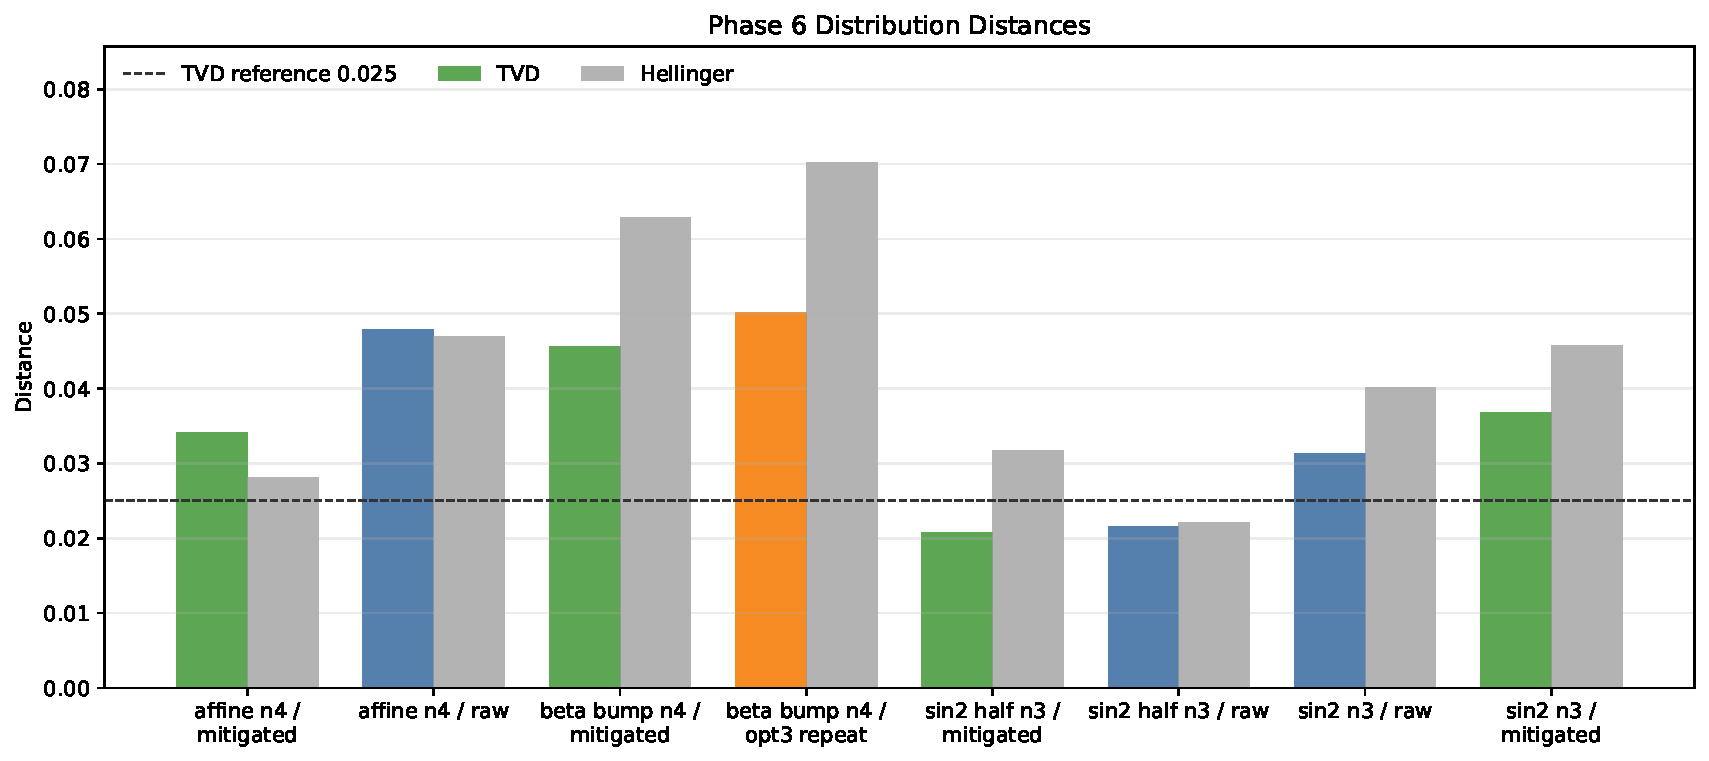
\includegraphics[width=\textwidth]{../results/phase6/figures/phase6_distribution_distances.pdf}
\caption{Phase 6 TVD and Hellinger distances for the available
Grover--Rudolph distribution measurements. TVD bar colors encode the
experimental variant: raw, mitigated, or opt-3 repeat. Hellinger bars are grey
to emphasize that they report a second distance metric for the same
case--variant pair, not a distinct hardware run.}
\label{fig:phase6-distribution-distances}
\end{figure}

The additional metrics confirm the Phase 5 interpretation. The mitigated affine
case improves across all reported distances. The opt-3 repeat of
\texttt{gr\_beta\_bump\_n4} lowers the Euclidean distance slightly but worsens
TVD, Hellinger distance, and classical fidelity. Therefore it is not a robust
improvement. Bootstrap analysis of quantities of interest also confirms that
the largest remaining errors are functional-specific, especially upper-half
events, moments, and \(\sin(\pi x)\) for selected profiles.

The purification diagnostic is simulator-only. It prepares \(p\) on a main
register, copies the computational-basis index to an auxiliary register with
CNOT gates, and measures both registers. In the ideal simulator, the two
marginals agree and the mismatch probability is zero. The first diagnostics use
6 qubits for the \(n=3\) profiles and 8 qubits for
\texttt{gr\_beta\_bump\_n4}. The observed simulator depths are 12, 13, and 28,
respectively, with zero mismatch. This provides a clean conceptual bridge
between Grover--Rudolph probability loading, algebraic probability, and
purification-based mixed-state preparation, without spending hardware credits.

The resulting decision table is shown in
Table~\ref{tab:phase6-decision-table}. The classification is deliberately
conservative: a profile is promoted only as a direct distribution result unless
the amplified Grover iterate has also passed the hardware stability tests.

\begin{table}[h]
\centering
\begin{tabular}{llrrl}
\toprule
Case & Variant & TVD & Max QoI err. & Decision \\
\midrule
\texttt{gr\_affine\_n4} & mitigated & 0.0341 & 0.0112
& selected direct functionals \\
\texttt{gr\_affine\_n4} & raw & 0.0479 & 0.0329
& diagnostic only \\
\texttt{gr\_beta\_bump\_n4} & mitigated & 0.0456 & 0.0177
& diagnostic only \\
\texttt{gr\_beta\_bump\_n4} & opt-3 repeat & 0.0502 & 0.0150
& diagnostic only \\
\texttt{gr\_sin2\_half\_n3} & mitigated & 0.0208 & 0.0186
& direct distribution \\
\texttt{gr\_sin2\_half\_n3} & raw & 0.0216 & 0.0196
& direct distribution \\
\texttt{gr\_sin2\_n3} & raw & 0.0313 & 0.0098
& direct distribution with caveat \\
\texttt{gr\_sin2\_n3} & mitigated & 0.0368 & 0.0178
& diagnostic only \\
\bottomrule
\end{tabular}
\caption{Phase 6 operational decisions from distribution and
quantity-of-interest postprocessing. No row is promoted to amplified QAE on the
current evidence.}
\label{tab:phase6-decision-table}
\end{table}

Table~\ref{tab:phase6-functional-decisions} gives the strongest direct
quantity-of-interest estimates selected across the available raw, mitigated,
and repeat variants. The table lists the test function \(f\in\mathcal{A}_n\);
the reported estimate is the algebraic-probability functional
\(I_{\hat p}(f)=\varphi_{\hat p}(f)\) evaluated on the measured frequency law,
and the exact value is \(I_p(f)=\varphi_p(f)\) evaluated on the target dyadic
law. These are the functionals that should be emphasized before any additional
hardware spending. Across the twenty selected case--functional pairs, five are
classified as publishable, seven as usable with a confidence interval, five as
usable only with an explicit bias report, and three as diagnostic.
Figure~\ref{fig:phase6-functional-errors} shows the full ordered
functional-error profile. Here the color convention changes because the plotted
object is different. Each bar is one selected functional \(I_{\hat p}(f)\), and
the height of the bar is the absolute error
\(|I_{\hat p}(f)-I_p(f)|\). The color does not encode the circuit variant; it
encodes the decision status assigned after comparing the error and the
bootstrap interval with the exact value. Green denotes publishable, blue
denotes usable with confidence-interval coverage, orange denotes usable only
with explicit bias reporting, purple denotes diagnostic, and red denotes
rejected. Thus the alternating colors in Figure~\ref{fig:phase6-functional-errors}
reflect the quality class of each functional, not an alternating sequence of
methods.

\begin{table}[h]
\centering
\begin{tabular}{llrrl}
\toprule
Case & Test function \(f\) & \(I_{\hat p}(f)\) & \(I_p(f)\) & Status \\
\midrule
\texttt{gr\_beta\_bump\_n4} & \(f(x)=x\)
& 0.28552 & 0.28434 & publishable \\
\texttt{gr\_sin2\_half\_n3} & \(f(x)=(x-1/2)_+\)
& 0.22211 & 0.22566 & publishable \\
\texttt{gr\_sin2\_half\_n3} & \(f(x)=\sin(\pi x)\)
& 0.64328 & 0.64073 & publishable \\
\texttt{gr\_sin2\_n3} & \(f(x)=(x-1/2)_+\)
& 0.07513 & 0.07571 & publishable \\
\texttt{gr\_sin2\_n3} & \(f(x)=x^2\)
& 0.28152 & 0.28274 & publishable \\
\bottomrule
\end{tabular}
\caption{Best Phase 6 direct quantity-of-interest functionals. The selected
variant is the one with the smallest absolute error in
\(|I_{\hat p}(f)-I_p(f)|\) among the available hardware runs.}
\label{tab:phase6-functional-decisions}
\end{table}

\begin{figure}[h]
\centering
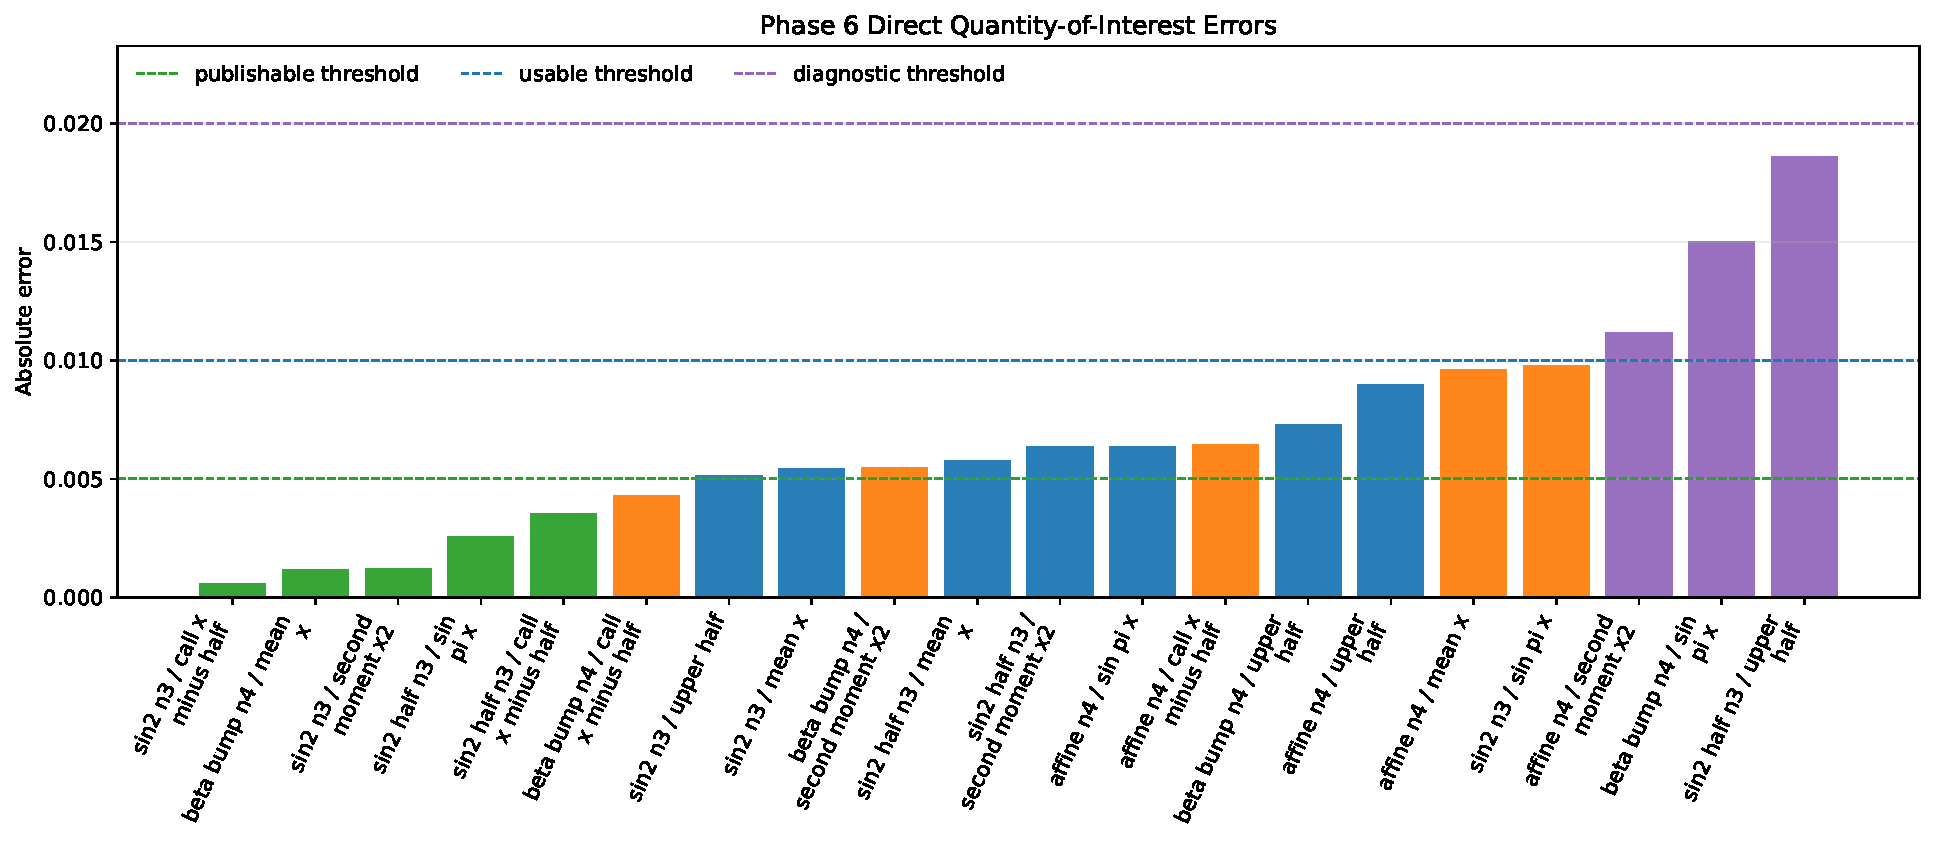
\includegraphics[width=\textwidth]{../results/phase6/figures/phase6_functional_errors.pdf}
\caption{Best direct quantity-of-interest errors selected across raw,
mitigated, and repeat variants. Bar colors encode the decision status assigned
to each functional: publishable, usable with confidence interval, usable with
explicit bias reporting, diagnostic, or rejected. The horizontal lines indicate
the publishable, usable, and diagnostic thresholds used by the Phase 6 decision
table.}
\label{fig:phase6-functional-errors}
\end{figure}

\subsection{Higher-shot validation of selected \(n=3\) distributions}

Phase 7 repeated the two \(n=3\) direct Grover--Rudolph distribution
measurements with 8192 shots and no Runtime mitigation. The purpose was not to
improve the global state-preparation claim by averaging alone, but to test
run-to-run stability of the finite probability law before escalating to deeper
amplified circuits. The result is summarized in
Table~\ref{tab:phase7-n3-validation}.

\begin{table}[h]
\centering
\begin{tabular}{lrrrrr}
\toprule
Case & Shots & TVD & Hellinger & Fidelity & Max. cell dev. \\
\midrule
\texttt{gr\_sin2\_half\_n3} & 8192 & 0.030093 & 0.035326 & 0.997506 & 0.022513 \\
\texttt{gr\_sin2\_n3} & 8192 & 0.056027 & 0.056296 & 0.993672 & 0.027206 \\
\texttt{gr\_affine\_n4} mitigated & 8192 & 0.028017 & 0.023874 & 0.998860 & 0.008197 \\
\bottomrule
\end{tabular}
\caption{Phase 7 higher-shot validation on \texttt{ibm\_fez}. The two \(n=3\)
runs are raw distribution measurements; the \texttt{gr\_affine\_n4} run uses
the same dynamical-decoupling and twirling options as the earlier mitigated
campaign. No Grover amplification or QAE circuit is used.}
\label{tab:phase7-n3-validation}
\end{table}

The higher-shot repeat does not reduce the discrepancy relative to the earlier
Phase 3 campaign. In particular, \texttt{gr\_sin2\_n3} crosses the predefined
TVD threshold of 0.04 and is therefore retained as diagnostic evidence rather
than promoted as a global distribution benchmark. The quantity-of-interest
analysis is more nuanced: \(I_p(x)\) for \texttt{gr\_sin2\_n3} remains
publishable with absolute error 0.001556, while
\(I_p((x-1/2)_+)\) and \(I_p(x^2)\) remain usable with explicit bias reporting.
For \texttt{gr\_sin2\_half\_n3}, the call payoff and \(\sin(\pi x)\)
functionals remain below \(10^{-2}\), but the upper-half event is rejected in
this repeat. This reinforces the central methodological conclusion: on current
hardware, direct Grover--Rudolph loading should be reported through
quantity-specific functionals \(I_{\hat p}(f)\), with run-to-run stability
checks, rather than as a blanket distribution-preparation success.

The mitigated \texttt{gr\_affine\_n4} repeat gives the cleanest Phase 7 global
distribution metric: TVD improves from 0.034112 in Phase 6 to 0.028017, and the
maximum cell deviation stays below \(10^{-2}\). The functional picture is again
more selective. The \(\sin(\pi x)\) functional remains usable with confidence
interval coverage and absolute error 0.006274, and the call payoff remains
below \(10^{-2}\) with explicit bias reporting. In contrast, \(I_p(x)\),
\(I_p(x^2)\), and the upper-half event are diagnostic or rejected in this
repeat, with the upper-half error increasing to 0.021078. Thus, even when
global distribution distances improve, the admissible conclusions remain tied
to the specific test function \(f\).

Combining the Phase 3 baseline, Phase 6 postprocessing, and Phase 7
higher-shot repeats gives the paper-quality classification in
Table~\ref{tab:phase7-paper-quality}. The classification is deliberately
conservative: a quantity is paper-quality only if the Phase 7 repeat either
preserves confidence-interval coverage or remains below \(10^{-2}\) with an
explicit bias caveat.

\begin{table}[h]
\centering
\begin{tabular}{lll}
\toprule
Category & Result & Decision \\
\midrule
Distribution & \texttt{gr\_affine\_n4} mitigated
& paper-quality distribution \\
\(I_p(f)\) & \texttt{gr\_affine\_n4}, \(f(x)=\sin(\pi x)\)
& paper-quality \\
\(I_p(f)\) & \texttt{gr\_sin2\_n3}, \(f(x)=x\)
& paper-quality \\
\(I_p(f)\) & \texttt{gr\_affine\_n4}, \(f(x)=(x-1/2)_+\)
& paper-quality with bias caveat \\
\(I_p(f)\) & \texttt{gr\_beta\_bump\_n4}, \(f(x)=(x-1/2)_+\)
& paper-quality with bias caveat \\
\(I_p(f)\) & \texttt{gr\_beta\_bump\_n4}, \(f(x)=x\)
& paper-quality with bias caveat \\
\(I_p(f)\) & \texttt{gr\_sin2\_half\_n3}, \(f(x)=(x-1/2)_+\)
& paper-quality with bias caveat \\
\(I_p(f)\) & \texttt{gr\_sin2\_half\_n3}, \(f(x)=\sin(\pi x)\)
& paper-quality with bias caveat \\
\(I_p(f)\) & \texttt{gr\_sin2\_n3}, \(f(x)=(x-1/2)_+\)
& paper-quality with bias caveat \\
\(I_p(f)\) & \texttt{gr\_sin2\_n3}, \(f(x)=x^2\)
& paper-quality with bias caveat \\
\bottomrule
\end{tabular}
\caption{Phase 3/6/7 classification of direct Grover--Rudolph hardware
evidence. Results not listed here are retained as backend diagnostics under the
current thresholds.}
\label{tab:phase7-paper-quality}
\end{table}

Figure~\ref{fig:phase7-distribution-classification} shows the final
distribution-level decision. The green bar is the only global distribution
claim retained for the paper-quality set. Purple bars are still scientifically
useful, but only as backend diagnostics: their full measured probability laws
are not stable enough for a global state-preparation claim on
\texttt{ibm\_fez}.

\begin{figure}[h]
\centering
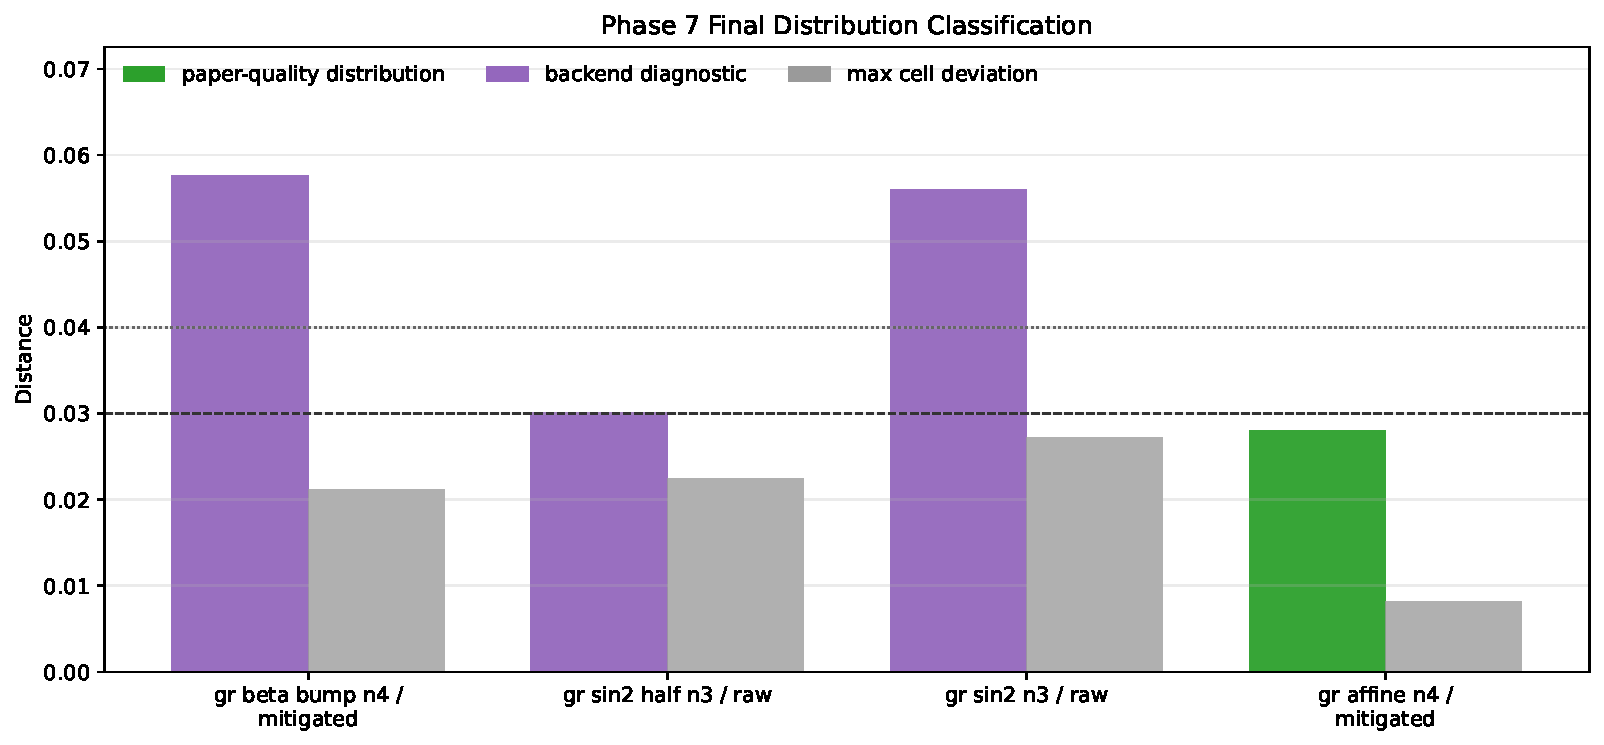
\includegraphics[width=\textwidth]{../results/phase7/figures/phase7_distribution_classification.pdf}
\caption{Final Phase 7 distribution-level classification. Bar height reports
TVD or maximum cell deviation. Color reports the final distribution decision:
paper-quality distribution or backend diagnostic distribution.}
\label{fig:phase7-distribution-classification}
\end{figure}

Figure~\ref{fig:phase7-qoi-classification} gives the corresponding
functional-level decision. This is the main paper-facing figure for the direct
Grover--Rudolph workflow: it separates quantities that are robust enough for the
main text, quantities that require explicit bias reporting, and quantities that
should remain backend diagnostics.

\begin{figure}[h]
\centering
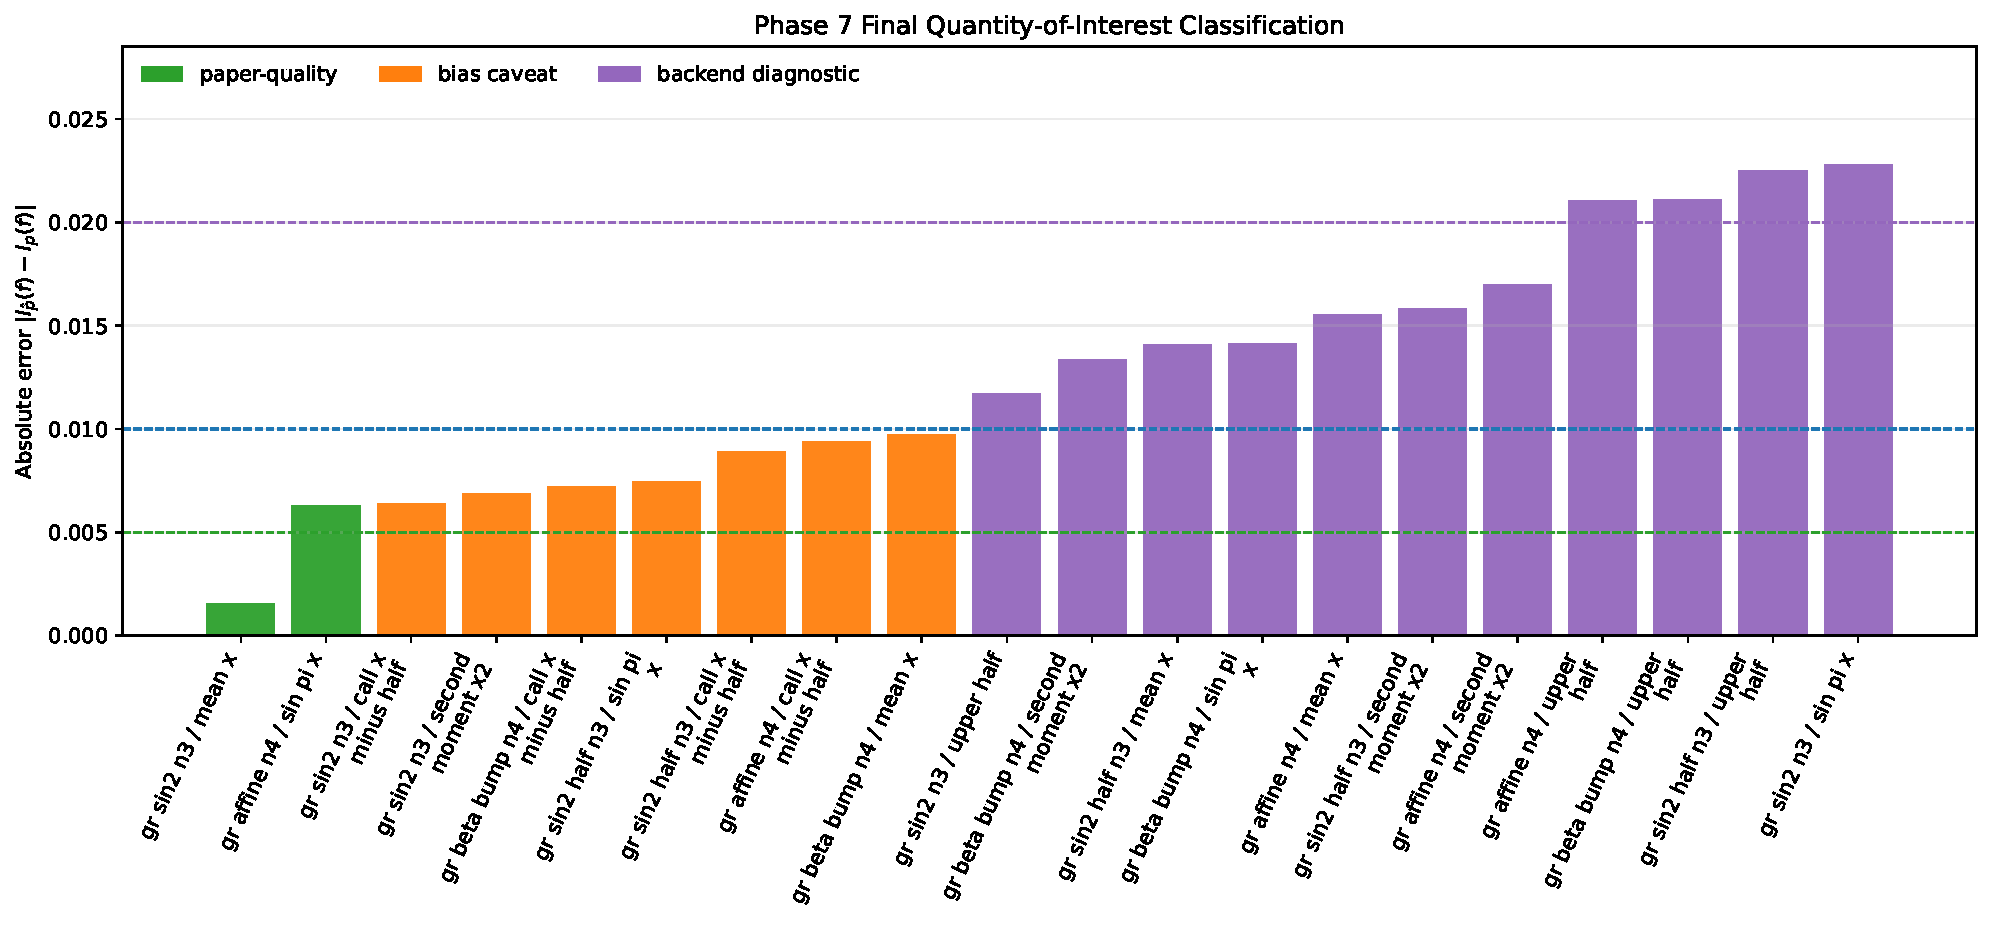
\includegraphics[width=\textwidth]{../results/phase7/figures/phase7_qoi_classification.pdf}
\caption{Final Phase 7 quantity-of-interest classification. Bar height is the
absolute functional error \(|I_{\hat p}(f)-I_p(f)|\). Color reports the final
decision class: paper-quality, paper-quality with explicit bias caveat, or
backend diagnostic.}
\label{fig:phase7-qoi-classification}
\end{figure}

The resulting publication narrative is therefore precise. The hardware evidence
supports one global distribution claim, namely the mitigated
\texttt{gr\_affine\_n4} loader, and a small set of quantity-specific
functionals. Several initially strong Phase 6 quantities degrade in Phase 7,
which makes them valuable diagnostics of backend drift rather than primary
numerical estimates. This distinction is central to the proposed methodology:
the experimental object is the finite probability state and the algebraic
functional \(I_p(f)\), with reproducibility assessed at the level of the
selected test function.

The final \texttt{gr\_beta\_bump\_n4} repeat removes the remaining pending
replication entries. Its global distribution error remains diagnostic
\((\mathrm{TVD}=0.057598)\), but two smooth or payoff-like functionals remain
below \(10^{-2}\): \(I_p(x)\), with absolute error 0.009738, and
\(I_p((x-1/2)_+)\), with absolute error 0.007214. The upper-half event does
not replicate and is rejected in this run, with absolute error 0.021095.

The run-to-run comparison in Figure~\ref{fig:phase7-qoi-error-change} explains
why the classification is conservative. Only two selected functionals improve
from Phase 6 to Phase 7, while most errors increase when the measurements are
repeated at higher shot count. This pattern points to backend drift and
functional-dependent bias rather than to simple sampling noise.

\begin{figure}[h]
\centering
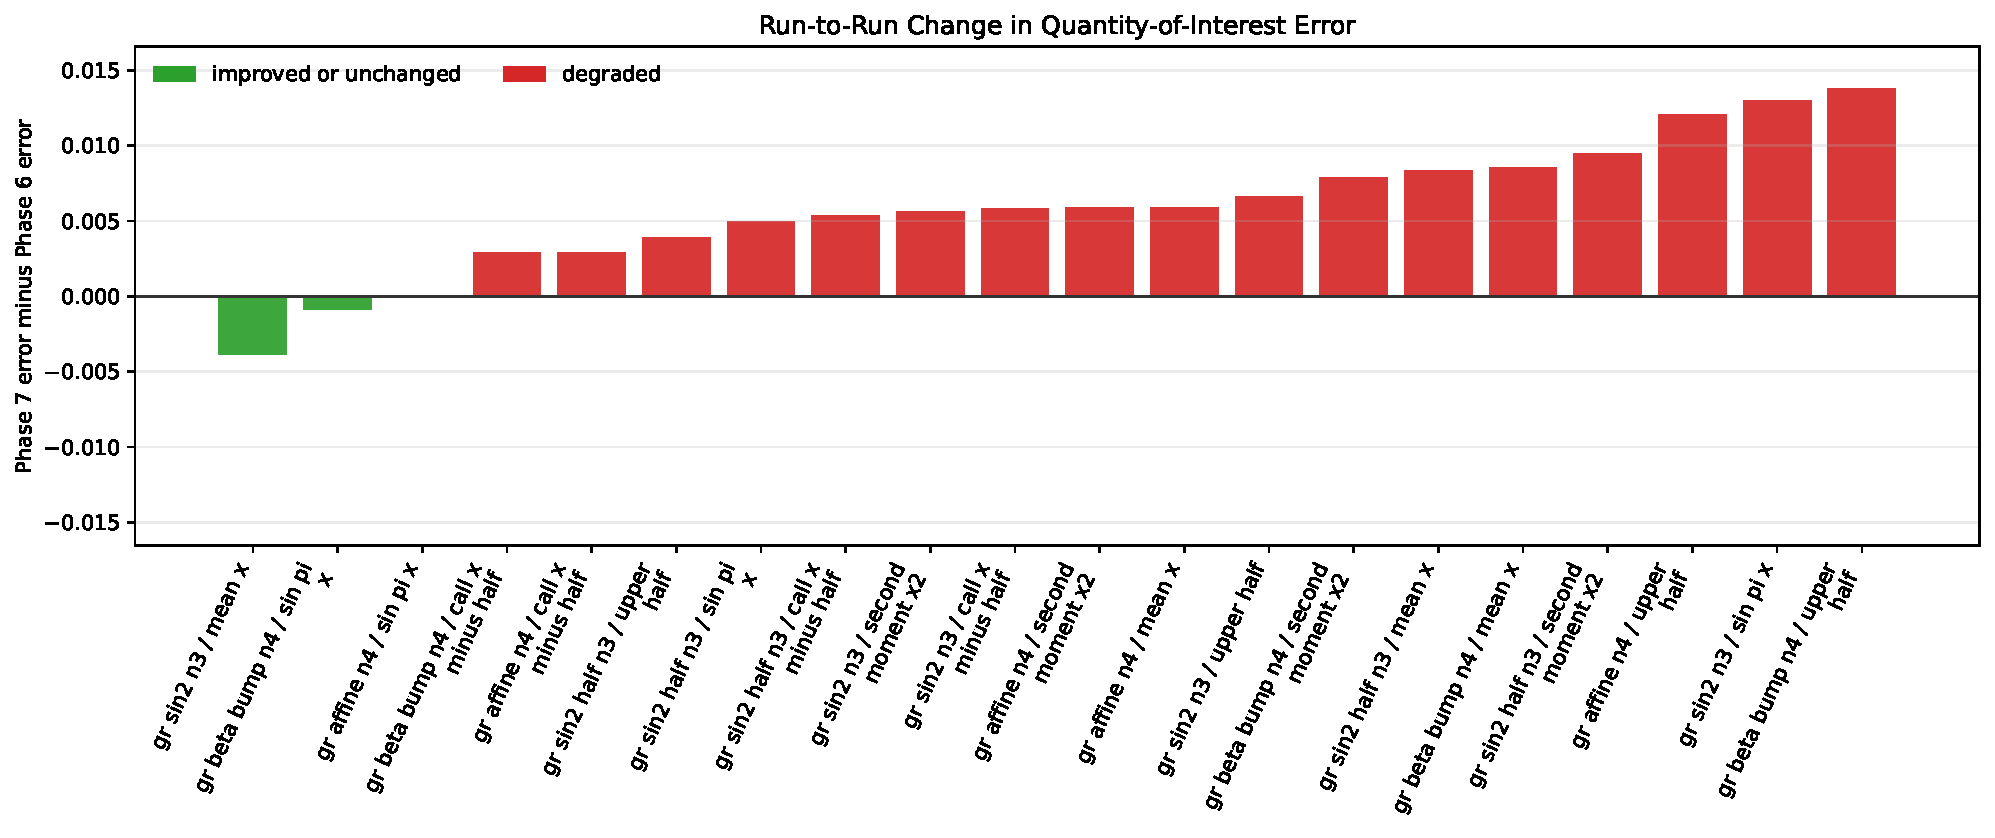
\includegraphics[width=\textwidth]{../results/phase7/figures/phase7_qoi_error_change.pdf}
\caption{Change in absolute quantity-of-interest error from Phase 6 to Phase 7.
Negative bars indicate improved or unchanged error; positive bars indicate
degradation in the higher-shot repeat.}
\label{fig:phase7-qoi-error-change}
\end{figure}

\subsection{Cross-backend validation on \texttt{ibm\_kingston}}

The first Phase 8 experiment repeats the strongest Phase 7 result on a second
backend. We selected the mitigated \texttt{gr\_affine\_n4} direct-distribution
campaign because it was the only global paper-quality distribution claim on
\texttt{ibm\_fez}. The \texttt{ibm\_kingston} backend has the same
\(\{\mathrm{cz},\mathrm{id},\mathrm{rz},\mathrm{sx},x\}\) basis family, but a
different calibration state, so it provides a clean cross-backend control
without changing the circuit family.

\begin{table}[h]
\centering
\begin{tabular}{lrrrr}
\toprule
Backend & TVD & Hellinger & \(F_{\mathrm{cl}}\) & Max. cell dev. \\
\midrule
\texttt{ibm\_fez} & 0.028017 & 0.023874 & 0.998860 & 0.008197 \\
\texttt{ibm\_kingston} & 0.021823 & 0.019060 & 0.999274 & 0.009195 \\
\bottomrule
\end{tabular}
\caption{Cross-backend Phase 8 validation of mitigated
\texttt{gr\_affine\_n4}. Both runs use 8192 shots, optimization level 2, and
the same dynamical-decoupling and twirling options.}
\label{tab:phase8-affine-cross-backend}
\end{table}

The Kingston run strengthens the main direct-distribution claim. Relative to
Fez, it improves TVD, Hellinger distance, classical fidelity, and Euclidean
distance, while keeping the maximum cell deviation below \(10^{-2}\).
Table~\ref{tab:phase8-affine-qoi-delta} shows that Kingston also reduces the
absolute error for every tested functional. The upper-half event remains
diagnostic, but its error falls from 0.021078 to 0.014486. The strongest
paper-quality functional, \(I_p(\sin(\pi x))\), improves from 0.006274 to
0.004731 and retains bootstrap interval coverage.

\begin{table}[h]
\centering
\begin{tabular}{lrrr}
\toprule
Test function \(f\) & Fez error & Kingston error & Change \\
\midrule
\((x-1/2)_+\) & 0.009374 & 0.004483 & -0.004891 \\
\(x\) & 0.015535 & 0.007235 & -0.008300 \\
\(x^2\) & 0.017012 & 0.008438 & -0.008574 \\
\(\sin(\pi x)\) & 0.006274 & 0.004731 & -0.001543 \\
\(1_{x\ge1/2}\) & 0.021078 & 0.014486 & -0.006592 \\
\bottomrule
\end{tabular}
\caption{Quantity-of-interest error changes for mitigated
\texttt{gr\_affine\_n4} when moving from \texttt{ibm\_fez} to
\texttt{ibm\_kingston}. Negative change means Kingston improves the absolute
error.}
\label{tab:phase8-affine-qoi-delta}
\end{table}

This result changes the status of the affine loader from a single-backend
success to cross-backend evidence. It also gives a useful warning for the next
Phase 8 submissions: the second backend can materially improve the same
compiled-depth and same-two-qubit-count circuit, so the remaining diagnostic
families should be tested on Kingston only when the scientific question is
backend dependence, not random repetition.

\subsection{Phase 9 integration-scaling audit}

The first Phase 9 run is a backend-aware, credit-free audit on
\texttt{ibm\_kingston}. It does not submit QPU jobs. It transpiles the
Grover--Rudolph loaders, simulates ideal shot noise, and uses the backend noise
model to estimate both global distribution error and the maximum
quantity-of-interest error over the selected functionals. The results are
summarized in Table~\ref{tab:phase9-first-audit}.

\begin{table}[h]
\centering
\begin{tabular}{lrrrrl}
\toprule
Case & Depth & 2q gates & Noisy TVD & Max. QoI err. & Status \\
\midrule
\texttt{gr\_sin2\_n3} & 31 & 7 & 0.028317 & 0.012576 & candidate \\
\texttt{gr\_sin2\_n4} & 62 & 16 & 0.029796 & 0.013991 & candidate \\
\texttt{gr\_beta\_bump\_n4} & 68 & 16 & 0.041681 & 0.007289 & candidate \\
\texttt{gr\_affine\_n4} & 74 & 16 & 0.028333 & 0.008659 & candidate \\
\texttt{gr\_beta\_bump\_n5} & 162 & 44 & 0.048994 & 0.014625 & candidate \\
\texttt{gr\_affine\_n5} & 171 & 44 & 0.044607 & 0.013084 & candidate \\
\texttt{gr\_sin2\_n5} & 141 & 44 & 0.052208 & 0.013443 & reject TVD \\
\bottomrule
\end{tabular}
\caption{First Phase 9 integration-scaling audit on \texttt{ibm\_kingston}.
The candidate threshold is noisy TVD below 0.05 and maximum
quantity-of-interest error below 0.02, in addition to depth and two-qubit-gate
limits.}
\label{tab:phase9-first-audit}
\end{table}

The audit gives a useful first ordering. The smooth symmetric \(n=5\) law is
rejected only by the noisy-TVD threshold, while its maximum functional error
remains below 0.02. The affine and localized \(n=5\) laws both pass the
predeclared thresholds. Among them, \texttt{gr\_affine\_n5} is the most natural
first hardware candidate because it refines the affine law already validated
across Fez and Kingston.

A focused layout and seed audit was then run for \texttt{gr\_affine\_n5}. The
best candidate uses optimization level 2 and transpiler seed 45678. It keeps the
same structural cost as the initial dry run, depth 171 and 44 two-qubit gates,
but improves the backend-noise prediction to TVD 0.025125 and maximum
quantity-of-interest error 0.005126. This is the configuration prepared for the
first Phase 9 hardware submission; no QPU job has been submitted at this stage.

The corresponding hardware run was then executed on \texttt{ibm\_kingston} with
8192 shots. The observed distribution metrics are shown in
Table~\ref{tab:phase9-affine-n5-hardware}. The measured TVD is larger than the
best noisy-model prediction, but it remains below the predeclared 0.05
threshold, and the maximum cell deviation remains below \(10^{-2}\).

\begin{table}[h]
\centering
\begin{tabular}{lrrrrrr}
\toprule
Case & Grid & Depth & 2q gates & TVD & Hellinger & Max. cell dev. \\
\midrule
\texttt{gr\_affine\_n5} & 32 & 171 & 44 & 0.033694 & 0.031298 & 0.008438 \\
\bottomrule
\end{tabular}
\caption{Phase 9 \texttt{gr\_affine\_n5} direct-distribution hardware result on
\texttt{ibm\_kingston}. The run uses Runtime mitigation, 8192 shots,
optimization level 2, and transpiler seed 45678.}
\label{tab:phase9-affine-n5-hardware}
\end{table}

The quantity-of-interest behavior is more selective, as summarized in
Table~\ref{tab:phase9-affine-n5-qoi}. The smooth test function
\(\sin(\pi x)\) remains the strongest result, with absolute error 0.003601 and
bootstrap interval coverage of the exact finite-law value. The call payoff is
below \(10^{-2}\) but lacks interval coverage. The mean, second moment, and
upper-half event show residual bias at the \(1.5\times 10^{-2}\) scale.

\begin{table}[h]
\centering
\begin{tabular}{lrrrrl}
\toprule
Test function \(f\) & Estimate & Exact & Error & CI contains exact & Status \\
\midrule
\(\sin(\pi x)\) & 0.640477 & 0.636876 & 0.003601 & yes & strongest \\
\((x-1/2)_+\) & 0.176748 & 0.185068 & 0.008320 & no & bias caveat \\
\(x\) & 0.605309 & 0.620136 & 0.014827 & no & diagnostic \\
\(x^2\) & 0.437745 & 0.453388 & 0.015642 & no & diagnostic \\
\(1_{x\ge1/2}\) & 0.663940 & 0.680380 & 0.016439 & no & diagnostic \\
\bottomrule
\end{tabular}
\caption{Phase 9 \texttt{gr\_affine\_n5} quantity-of-interest estimates from
the measured 32-cell probability law.}
\label{tab:phase9-affine-n5-qoi}
\end{table}

This is the first positive 32-cell scaling result in the project. It supports
the direct Grover--Rudolph distribution workflow beyond the 16-cell affine
anchor, but it also confirms that integration claims must remain
quantity-specific. The hardware result should therefore be reported as a
paper-quality distribution-scaling result, with \(\sin(\pi x)\) as the cleanest
associated functional and the tail/moment quantities retained as backend-bias
diagnostics.

The next credit-free Phase 9 audit targeted the localized 32-cell law
\texttt{gr\_beta\_bump\_n5}. This is a stress case because localized
probability mass was less stable in the earlier \(n=4\) campaigns. A layout and
seed search on \texttt{ibm\_kingston} selected optimization level 2 and
transpiler seed 67890. The prepared circuit has depth 162, 44 two-qubit gates,
and two-qubit depth 42. The backend-noise prediction is TVD 0.032691 and
maximum quantity-of-interest error 0.004585. This makes
\texttt{gr\_beta\_bump\_n5} the next prepared hardware candidate.

The hardware result did not confirm the optimistic noisy-model prediction. The
measured TVD is 0.073298, with Hellinger distance 0.110712 and classical
fidelity 0.975636. The maximum cell deviation remains moderate, 0.014583, but
the global shape error is above the predeclared Phase 9 threshold. The
quantity-of-interest errors also fail to show a clean functional result:
\((x-1/2)_+\) has error 0.012934, \(x\) has error 0.020770, \(x^2\) has error
0.024336, \(\sin(\pi x)\) has error 0.013662, and the upper-half event has
error 0.037838; none of the bootstrap intervals contains the exact finite-law
value.

\begin{table}[h]
\centering
\small
\begin{tabular}{lrrrrl}
\toprule
Case & Depth & 2q gates & TVD & Max. dev. & Decision \\
\midrule
\texttt{gr\_affine\_n5} & 171 & 44 & 0.033694 & 0.008438
& paper-quality \\
\texttt{gr\_beta\_bump\_n5} & 162 & 44 & 0.073298 & 0.014583
& diagnostic \\
\bottomrule
\end{tabular}
\caption{Phase 9 closing comparison for 32-cell direct Grover--Rudolph
distribution loading on \texttt{ibm\_kingston}.}
\label{tab:phase9-closing-comparison}
\end{table}

Phase 9 therefore gives a sharp boundary. The affine law scales successfully
from 16 to 32 cells under the direct distribution workflow, while the localized
beta-like law does not. This is not a failure of the experimental program; it
identifies localized probability structure as the next limiting regime for
current hardware and mitigation settings.

\subsection{Phase 10 comparison with MC/QMC sampling}

Phase 10 uses the two Phase 9 32-cell hardware distributions and compares them
with MC and randomized QMC sampling from the same finite law, using the same
sample count \(M=8192\). The distribution-level comparison is shown in
Table~\ref{tab:phase10-distribution-baselines}. The QPU TVD for
\texttt{gr\_affine\_n5} is above the MC median but still at the same order of
magnitude. The \texttt{gr\_beta\_bump\_n5} TVD is far outside the MC sampling
scale. The QMC baseline is much sharper because it uses the exact finite inverse
CDF; it is therefore a reference baseline once \(p\) is known.
Figure~\ref{fig:phase10-distribution-baselines} visualizes the same comparison:
blue bars are the QPU empirical TVD, orange bars are the MC median TVD, and
green bars are the randomized QMC median TVD.

\begin{table}[h]
\centering
\small
\begin{tabular}{lrrrrr}
\toprule
Case & QPU & MC med. & QMC med. & Rank MC & Rank QMC \\
\midrule
\texttt{gr\_affine\_n5} & 0.033694 & 0.023578 & 0.000634 & 0.997 & 1.000 \\
\texttt{gr\_beta\_bump\_n5} & 0.073298 & 0.020190 & 0.000632 & 1.000 & 1.000 \\
\bottomrule
\end{tabular}
\caption{Phase 10 distribution-level sampling comparison. Percentile ranks
report the fraction of MC/QMC trials whose TVD is no larger than the QPU TVD.}
\label{tab:phase10-distribution-baselines}
\end{table}

\begin{figure}[h]
\centering
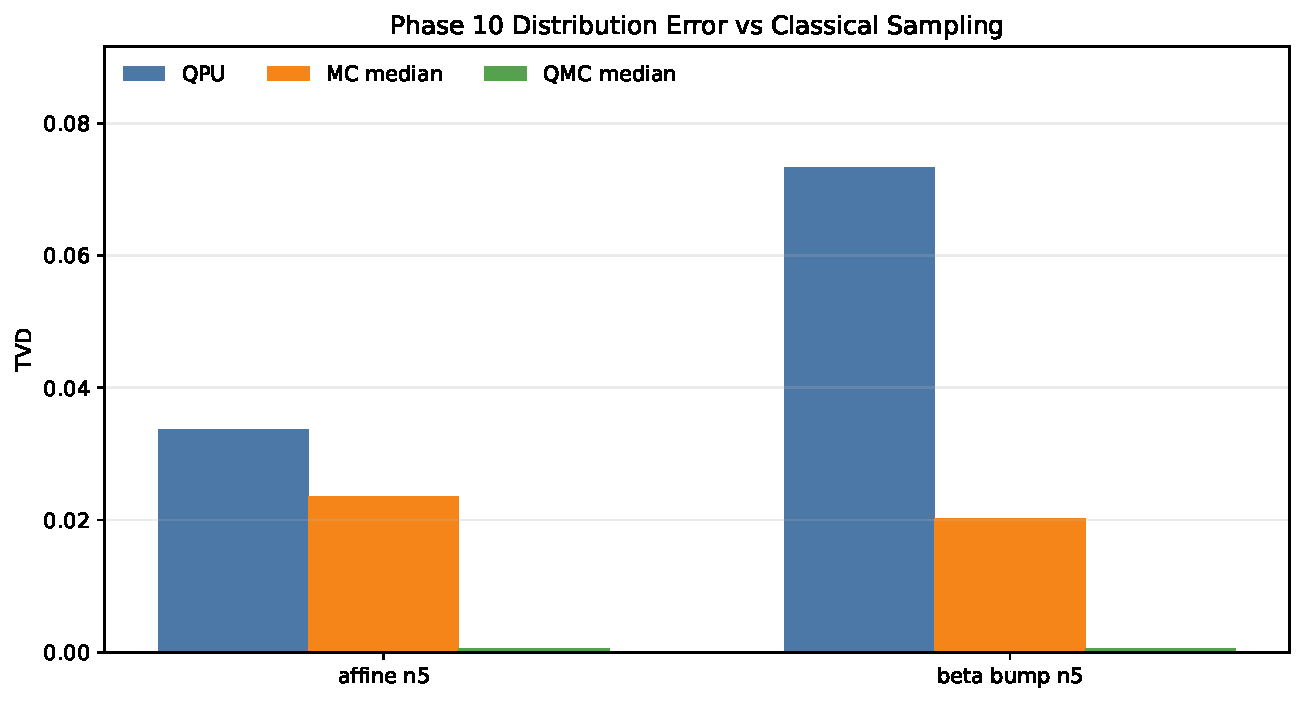
\includegraphics[width=0.86\linewidth]{../results/phase10/figures/phase10_distribution_sampling_baselines.pdf}
\caption{Phase 10 distribution-level comparison against MC and QMC sampling
from the same finite probability laws.}
\label{fig:phase10-distribution-baselines}
\end{figure}

The quantity-of-interest comparison is more nuanced. For
\texttt{gr\_affine\_n5}, \(I_p(\sin(\pi x))\) remains the only estimate at the
MC sampling scale: its QPU error is 0.003601, compared with MC RMSE 0.003294.
All other tested quantities have QPU errors between 3 and 5 times the
corresponding MC RMSE. For \texttt{gr\_beta\_bump\_n5}, every tested quantity is
substantially worse than MC, confirming that this case should be reported as a
localized-profile stress diagnostic. Table~\ref{tab:phase10-qoi-baselines}
lists representative rows.
Figure~\ref{fig:phase10-qoi-baselines} uses color to encode the decision status:
green denotes MC-competitive, orange denotes hardware-bias diagnostic, red
denotes MC-dominated, and gray denotes the MC RMSE baseline.

\begin{table}[h]
\centering
\begin{tabular}{llrrrr}
\toprule
Case & Test function \(f\) & QPU error & MC RMSE & QMC RMSE & QPU/MC \\
\midrule
\texttt{gr\_affine\_n5} & \(\sin(\pi x)\) & 0.003601 & 0.003294 & \(\approx 0\) & 1.09 \\
\texttt{gr\_affine\_n5} & \((x-1/2)_+\) & 0.008320 & 0.001882 & 0.000019 & 4.42 \\
\texttt{gr\_affine\_n5} & \(x\) & 0.014827 & 0.002870 & 0.000037 & 5.17 \\
\texttt{gr\_affine\_n5} & \(1_{x\ge1/2}\) & 0.016439 & 0.005177 & 0.000057 & 3.18 \\
\texttt{gr\_beta\_bump\_n5} & \((x-1/2)_+\) & 0.012934 & 0.000413 & 0.000017 & 31.34 \\
\texttt{gr\_beta\_bump\_n5} & \(\sin(\pi x)\) & 0.013662 & 0.002793 & 0.000013 & 4.89 \\
\texttt{gr\_beta\_bump\_n5} & \(1_{x\ge1/2}\) & 0.037838 & 0.003464 & 0.000021 & 10.92 \\
\bottomrule
\end{tabular}
\caption{Phase 10 quantity-of-interest comparison against MC/QMC sampling from
the same finite probability law with \(M=8192\). The near-zero QMC RMSE for
\(\sin(\pi x)\) in the affine case is a finite-grid effect of inverse-CDF QMC,
and should not be interpreted as a full cost model.}
\label{tab:phase10-qoi-baselines}
\end{table}

\begin{figure}[h]
\centering
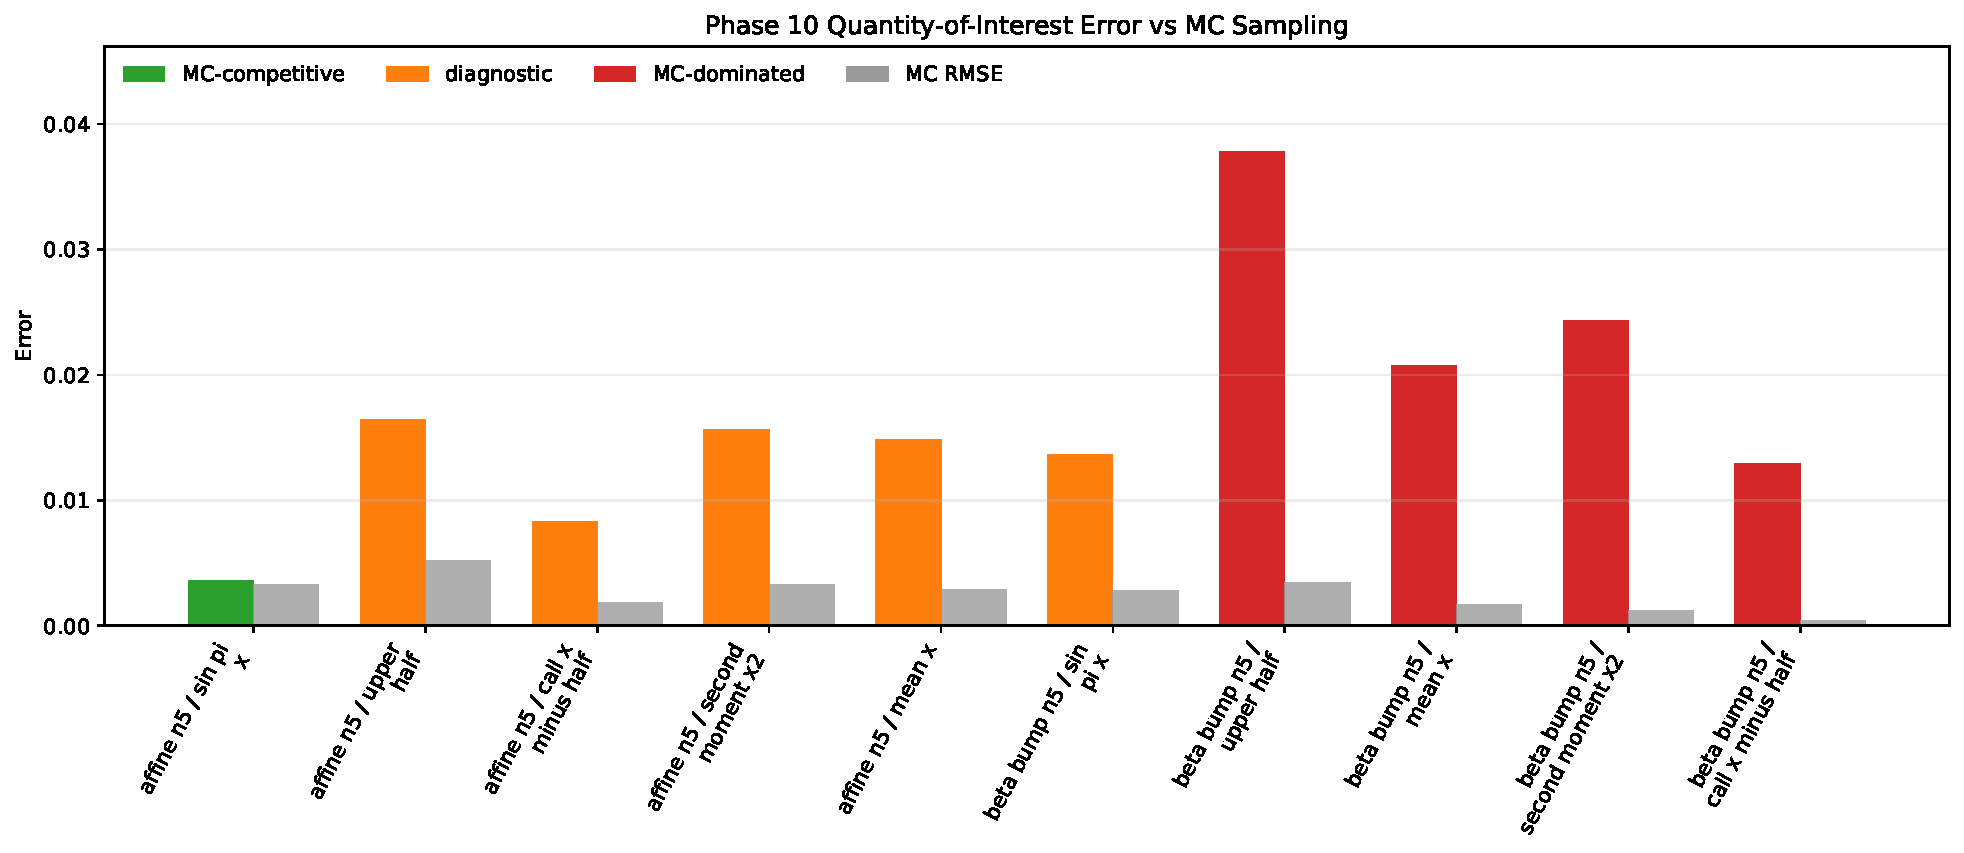
\includegraphics[width=0.98\linewidth]{../results/phase10/figures/phase10_qoi_sampling_baselines.pdf}
\caption{Phase 10 quantity-of-interest comparison. Colored bars are QPU
absolute errors, and gray bars are MC RMSE at the same sample count.}
\label{fig:phase10-qoi-baselines}
\end{figure}

\subsection{Phase 11 dual angle-structure decisions}

Phase 11 combines the structural angle classes with the Phase 9 and Phase 10
evidence. The resulting table is not a new hardware result; it is a
credit-free policy for what should be attempted next. The most important rows
are listed in Table~\ref{tab:phase11-dual-angle-decisions}. They show that the
only current paper-quality direct integral remains the 32-cell affine law with
\(f(x)=\sin(\pi x)\). Low-angle quantities for the \(\sin^2(\pi x)\) profiles
are the natural simulator candidates for amplified QAE. Localized beta-like
tail quantities are deferred because Phase 10 already shows MC-dominated
hardware error.

\begin{table}[h]
\centering
\small
\begin{tabular}{lllll}
\toprule
Case & Test function \(f\) & Profile class & \(f\) class & Recommendation \\
\midrule
\texttt{gr\_affine\_n5} & \(\sin(\pi x)\) & \(\mathcal{G}^{(5)}_5\) & \(\mathcal{G}^{(4)}_5\) & paper-quality direct \\
\texttt{gr\_sin2\_n3} & \(1_{x\ge1/2}\) & \(\mathcal{G}^{(2)}_3\) & \(\mathcal{G}^{(1)}_3\) & simulate QAE \\
\texttt{gr\_sin2\_n3} & \(\sin(\pi x)\) & \(\mathcal{G}^{(2)}_3\) & \(\mathcal{G}^{(2)}_3\) & simulate QAE \\
\texttt{gr\_sin2\_n4} & \(1_{x\ge1/2}\) & \(\mathcal{G}^{(2)}_4\) & \(\mathcal{G}^{(1)}_4\) & simulate QAE \\
\texttt{gr\_affine\_n5} & \(1_{x\ge1/2}\) & \(\mathcal{G}^{(5)}_5\) & \(\mathcal{G}^{(1)}_5\) & simulator only \\
\texttt{gr\_beta\_bump\_n5} & \(1_{x\ge1/2}\) & \(\mathcal{G}^{(5)}_5\) & \(\mathcal{G}^{(1)}_5\) & defer QPU repeat \\
\texttt{gr\_beta\_bump\_n5} & \((x-1/2)_+\) & \(\mathcal{G}^{(5)}_5\) & \(\mathcal{G}^{(5)}_5\) & defer QPU repeat \\
\bottomrule
\end{tabular}
\caption{Phase 11 dual angle-structure decisions. The profile class concerns
the law-defining profile \(F\) interpreted as an amplitude function; the
function class concerns the test function \(f\).}
\label{tab:phase11-dual-angle-decisions}
\end{table}

The practical implication is that angle degree is a filter, not a verdict. Low
angle degree is sufficient to justify simulator-level amplified-QAE studies,
but it does not override measured hardware bias. High angle degree does not
forbid direct Grover--Rudolph integration, but it is a warning against
immediately recasting the same quantity as an amplified-QAE amplitude.

\subsection{Phase 12 local QAE-amplitude audit}

Phase 12 constructs the actual amplitude-estimation circuits for the Phase 11
QAE candidates. The augmented state preparation loads the finite law \(p\) on
the grid register and the test function \(f\) on one objective qubit, so that
the marked probability is \(a=I_p(f)\). The exact statevector probabilities
match \(p_k(a)\) to numerical precision; the maximum discrepancy across the
audit is \(2.4\times 10^{-14}\). The relevant outcome is therefore not logical
correctness, but schedule informativeness and transpiled cost.

\begin{table}[h]
\centering
\small
\begin{tabular}{llrrrl}
\toprule
Case & Test function \(f\) & \(a=I_p(f)\) & Max. \(k\) & 2q gates & Recommendation \\
\midrule
\texttt{gr\_sin2\_n3} & \(1_{x\ge1/2}\) & 0.500000 & 2 & 35 & degenerate \\
\texttt{gr\_sin2\_n4} & \(1_{x\ge1/2}\) & 0.500000 & 2 & 87 & degenerate \\
\texttt{gr\_affine\_n5} & \(1_{x\ge1/2}\) & 0.680380 & 1 & 113 & \(k=1\) depth watch \\
\texttt{gr\_sin2\_n3} & \(\sin(\pi x)\) & 0.848596 & 2 & 86 & simulator candidate \\
\bottomrule
\end{tabular}
\caption{Phase 12 local audit of augmented QAE amplitude circuits. The two
upper-half \(\sin^2(\pi x)\) cases have low angle degree but are not
informative for QAE because \(a=1/2\), hence \(p_k(a)=1/2\) for all \(k\).}
\label{tab:phase12-qae-amplitude-audit}
\end{table}

This result sharpens the Phase 11 policy. Angle class is necessary for
candidate selection, but it must be combined with the scalar amplitude value
and the amplified schedule. The only non-degenerate local QAE candidate in this
audit is \texttt{gr\_sin2\_n3} with \(f(x)=\sin(\pi x)\), which reaches
\(k=2\) with 86 two-qubit gates after local \texttt{cz}-basis transpilation.
The 32-cell affine upper-half pair has useful amplification contrast, but only
passes through \(k=1\) under the current thresholds and is therefore not a QPU
candidate yet.

\subsection{Phase 13 backend-aware noisy QAE audit}

The only non-degenerate Phase 12 QAE candidate,
\texttt{gr\_sin2\_n3} with \(f(x)=\sin(\pi x)\), was then tested with
backend-derived noisy simulation. The audit was run on both
\texttt{ibm\_kingston} and \texttt{ibm\_fez}. No QPU jobs were submitted. The
local basis-only circuit reaches \(k=2\) with depth 288 and 86 two-qubit gates,
but the backend-aware transpilation/noise audit rejects a full
\(K=\{0,1,2\}\) hardware schedule.

\begin{table}[h]
\centering
\small
\begin{tabular}{llrrrrr}
\toprule
Backend & \(k\) & Depth & 2q gates & Expected \(p_k\) & Noisy \(p_k\) & Dev. \\
\midrule
\texttt{ibm\_kingston} & 0 & 68 & 20 & 0.848596 & 0.494873 & 0.353723 \\
\texttt{ibm\_kingston} & 1 & 222 & 63 & 0.131990 & 0.491211 & 0.359221 \\
\texttt{ibm\_fez} & 0 & 60 & 18 & 0.848596 & 0.501953 & 0.346643 \\
\texttt{ibm\_fez} & 1 & 292 & 83 & 0.131990 & 0.477783 & 0.345793 \\
\bottomrule
\end{tabular}
\caption{Phase 13 backend-aware noisy audit for the augmented QAE candidate
\texttt{gr\_sin2\_n3}, \(f(x)=\sin(\pi x)\). Both backends collapse the marked
probabilities toward roughly one half, and \(k=2\) is not retained under the
current cost thresholds.}
\label{tab:phase13-qae-noisy-audit}
\end{table}

This is decisive negative evidence before spending credits. The candidate is
logically correct and structurally meaningful, but current backend noise makes
the amplified probability model unusable. The project should therefore keep
augmented QAE in the simulator/noisy-audit track and continue using direct
Grover--Rudolph distribution sampling as the hardware-facing workflow.

\subsection{Phase 14 local scaling audit for direct integration}

The next local audit compares direct Grover--Rudolph sampling from \(n=4\) to
\(n=6\) before any backend decision. Table~\ref{tab:phase14-direct-scaling}
summarizes the best local \texttt{cz}-basis transpilation over the tested
optimization levels and seeds. The class column refers to the positive profile
after rescaling to \([0,1]\), used only as an angle-structure diagnostic.

\begin{table}[h]
\centering
\small
\begin{tabular}{lrrrrr}
\toprule
Case & \(n\) & Grid & Class & Depth & 2q gates \\
\midrule
\texttt{gr\_sin2\_n4} & 4 & 16 & \(\mathcal{G}^{(4)}_4\) & 52 & 14 \\
\texttt{gr\_sin2\_n5} & 5 & 32 & \(\mathcal{G}^{(4)}_5\) & 102 & 30 \\
\texttt{gr\_sin2\_n6} & 6 & 64 & \(\mathcal{G}^{(6)}_6\) & 200 & 62 \\
\texttt{gr\_affine\_n4} & 4 & 16 & \(\mathcal{G}^{(4)}_4\) & 69 & 14 \\
\texttt{gr\_affine\_n5} & 5 & 32 & \(\mathcal{G}^{(5)}_5\) & 141 & 30 \\
\texttt{gr\_affine\_n6} & 6 & 64 & \(\mathcal{G}^{(6)}_6\) & 287 & 62 \\
\texttt{gr\_beta\_bump\_n4} & 4 & 16 & \(\mathcal{G}^{(4)}_4\) & 61 & 14 \\
\texttt{gr\_beta\_bump\_n5} & 5 & 32 & \(\mathcal{G}^{(5)}_5\) & 125 & 30 \\
\texttt{gr\_beta\_bump\_n6} & 6 & 64 & \(\mathcal{G}^{(6)}_6\) & 253 & 62 \\
\bottomrule
\end{tabular}
\caption{Phase 14 local direct-sampling scaling audit. All rows pass the local
cost and discretization thresholds and are therefore candidates for a later
backend-aware audit. This table does not imply QPU submission.}
\label{tab:phase14-direct-scaling}
\end{table}

The local result is encouraging but deliberately limited. Moving from 32 to 64
midpoint cells roughly doubles the two-qubit count from 30 to 62 in this local
basis-only transpilation, while the worst midpoint discretization error across
the tested quantities remains below \(3.3\times10^{-3}\) for \(n=4\) and below
\(2.1\times10^{-4}\) for the \(n=6\) rows. Thus no \(n=6\) direct-sampling
candidate is rejected locally. However, Phase 9 already showed that localized
profiles can fail on hardware despite moderate circuit size. The proper next
step is therefore a backend-aware layout/noise audit for these \(n=6\) rows,
followed by at most one carefully selected QPU campaign.

That backend-aware audit was performed for the three \(n=6\) rows on both
\texttt{ibm\_kingston} and \texttt{ibm\_fez}, still without submitting QPU
jobs. Table~\ref{tab:phase14-backend-scaling} reports the best transpiled
candidate for each backend and the noisy simulation diagnostics.

\begin{table}[h]
\centering
\small
\begin{tabular}{llrrrrl}
\toprule
Backend & Case & Depth & 2q gates & Noisy TVD & Max QoI err. & Status \\
\midrule
\texttt{ibm\_kingston} & \texttt{gr\_sin2\_n6} & 294 & 103 & 0.057414 & 0.024009 & candidate \\
\texttt{ibm\_kingston} & \texttt{gr\_affine\_n6} & 361 & 103 & 0.046682 & 0.014242 & candidate \\
\texttt{ibm\_kingston} & \texttt{gr\_beta\_bump\_n6} & 338 & 103 & 0.047766 & 0.009092 & candidate \\
\texttt{ibm\_fez} & \texttt{gr\_sin2\_n6} & 299 & 103 & 0.069657 & 0.034643 & hold \\
\texttt{ibm\_fez} & \texttt{gr\_affine\_n6} & 361 & 103 & 0.048864 & 0.028890 & hold \\
\texttt{ibm\_fez} & \texttt{gr\_beta\_bump\_n6} & 337 & 103 & 0.059496 & 0.017425 & candidate \\
\bottomrule
\end{tabular}
\caption{Phase 14 backend-aware direct-sampling audit for the \(n=6\)
candidates. The status is a pre-submission decision from noisy simulation and
layout-aware transpilation; no QPU jobs are submitted by this audit.}
\label{tab:phase14-backend-scaling}
\end{table}

The most coherent next hardware test is therefore not the row with the lowest
single noisy quantity error, but the row that extends the existing
paper-quality line of evidence. The recommended microcampaign is
\texttt{gr\_affine\_n6} on \texttt{ibm\_kingston}. It extends the successful
32-cell affine result to 64 cells and remains below the noisy TVD and
quantity-of-interest error thresholds. The localized beta-like row remains a
stress diagnostic because Phase 9 already showed that this family can look
reasonable in pre-submission audits while failing as a clean integration result
on hardware.

The selected \texttt{gr\_affine\_n6} microcampaign was then executed on
\texttt{ibm\_kingston} with 8192 shots, dynamical decoupling, and twirling. The
measured distribution has TVD 0.058478 and maximum cell deviation 0.004792,
using a depth-361 circuit with 103 two-qubit gates. This passes the Phase 14
distribution rule, but the quantity-of-interest estimates in
Table~\ref{tab:phase14-affine-n6-qoi} show a strong functional dependence.

\begin{table}[h]
\centering
\small
\begin{tabular}{lrrrrl}
\toprule
Quantity of interest & Estimate & Exact & Error & 95\% CI contains exact & Status \\
\midrule
\(\sin(\pi x)\) & 0.637435 & 0.636684 & 0.000752 & yes & paper-quality \\
\((x-1/2)_+\) & 0.168151 & 0.185112 & 0.016961 & no & diagnostic \\
\(x\) & 0.586767 & 0.620224 & 0.033457 & no & diagnostic \\
\(x^2\) & 0.419880 & 0.453537 & 0.033657 & no & diagnostic \\
\(1_{x\ge 1/2}\) & 0.630249 & 0.680380 & 0.050131 & no & diagnostic \\
\bottomrule
\end{tabular}
\caption{Phase 14 quantity-of-interest estimates from the 64-cell affine
Grover--Rudolph distribution measured on \texttt{ibm\_kingston}.}
\label{tab:phase14-affine-n6-qoi}
\end{table}

Compared with the earlier 32-cell affine result, the distribution TVD increases
from 0.033694 to 0.058478. Nevertheless, the most robust integration quantity,
\(I_p(\sin(\pi x))\), improves from absolute error 0.003601 to 0.000752 and is
statistically compatible with the exact finite-law value. The tail and moment
quantities become worse and remain backend-bias diagnostics. Thus the correct
Phase 14 claim is not a uniform improvement from \(n=5\) to \(n=6\), but a
stronger paper-quality result for the smooth quantity \(I_p(\sin(\pi x))\) on a
64-cell law.

\subsection{Phase 15 centered Gaussian finite-law test}

The Phase 15 backend-aware audit selected the broad centered Gaussian-like
profile \(\sigma=0.25\) as the best alternative \(n=6\) probability law on
\texttt{ibm\_kingston}. The selected circuit had depth 193 and 66 two-qubit
gates, substantially below the affine \(n=6\) circuit. The noisy pre-submission
model predicted TVD 0.044257 and maximum quantity-of-interest error 0.012389.

The QPU execution gives TVD 0.070511 and maximum cell deviation 0.005211. Thus
the distribution shape is not globally better than the affine \(n=6\) result,
but the quantity-of-interest behaviour is complementary, as shown in
Table~\ref{tab:phase15-gaussian-qoi}.

\begin{table}[h]
\centering
\small
\begin{tabular}{lrrrrl}
\toprule
Quantity of interest & Estimate & Exact & Error & 95\% CI contains exact & Status \\
\midrule
\(1_{x\ge 1/2}\) & 0.496338 & 0.500000 & 0.003662 & yes & validation \\
\(x\) & 0.496075 & 0.500000 & 0.003925 & yes & validation \\
\(x^2\) & 0.304913 & 0.298362 & 0.006552 & no & diagnostic \\
\((x-1/2)_+\) & 0.098776 & 0.090369 & 0.008407 & no & diagnostic \\
\(\sin(\pi x)\) & 0.738914 & 0.782703 & 0.043789 & no & diagnostic \\
\bottomrule
\end{tabular}
\caption{Phase 15 quantity-of-interest estimates from the 64-cell centered
Gaussian-like Grover--Rudolph distribution measured on \texttt{ibm\_kingston}.}
\label{tab:phase15-gaussian-qoi}
\end{table}

This closes the direct finite-law block with a deliberately non-uniform
conclusion. The affine \(n=6\) law remains the best result for the smooth
quantity \(I_p(\sin(\pi x))\), with error 0.000752. The centered Gaussian-like
law gives better estimates for the upper-half mass and the mean, both with
interval coverage, but it fails badly for \(I_p(\sin(\pi x))\). The relevant
lesson is therefore not that one probability law is uniformly superior; it is
that the hardware bias couples strongly to both the prepared law \(p\) and the
chosen test function \(f\).

\subsection{Bridge to quadrature-rule QAE integration}

The preceding phases study finite-law integration after probability-law
preparation. This workflow estimates \(I_p(f)\) from measured frequencies and
is well suited to testing Grover--Rudolph state preparation on hardware. The
angle-structure paper, however, formulates numerical integration differently:
the integrand \(g\) is encoded as an amplitude, and the numerical rule is one
of the left Riemann, midpoint, right Riemann, or Simpson quadrature schemes.
The next experimental block should therefore return to that formulation and
measure
\[
  I[g]-\widehat Q_n^{(p)}[g]
  =
  \bigl(I[g]-Q_n^{(p)}[g]\bigr)
  +
  \bigl(Q_n^{(p)}[g]-\widehat Q_n^{(p)}[g]\bigr),
\]
separating discretization error from QAE/MLAE estimation error.

\subsection{Phase 15b quadrature-rule QAE hardware results}
\label{subsec:phase15b-quadrature-results}

The \texttt{ibm\_kingston} midpoint-quadrature microcampaign completed with all
ten submitted jobs in the \texttt{DONE} state. Table~\ref{tab:phase15b-results}
summarizes the grouped MLAE estimates. The reported quadrature value
\(Q_n[g]\) is the exact midpoint rule value on the selected grid; the true value
\(I[g]\) is the high-accuracy classical reference integral.

\begin{table}[h]
\centering
\begin{tabular}{lrrrrr}
\toprule
Case & \(Q_n[g]\) & \(I[g]\) & \(\widehat Q_n[g]\) & Est. err. & Total err. \\
\midrule
\texttt{g1\_n2\_midpoint} & 0.500000 & 0.500000 & 0.498828 & 0.001172 & 0.001172 \\
\texttt{g2\_n2\_midpoint} & 0.500000 & 0.500000 & 0.500140 & 0.000140 & 0.000140 \\
\texttt{affine\_shifted\_n2\_midpoint} & 0.395000 & 0.395000 & 0.405640 & 0.010640 & 0.010640 \\
\texttt{smooth\_bump\_n3\_midpoint} & 0.033974 & 0.033333 & 0.034902 & 0.000928 & 0.001568 \\
\bottomrule
\end{tabular}
\caption{Phase 15b midpoint-quadrature MLAE estimates from
\texttt{ibm\_kingston}. ``Est. err.'' is
\(|\widehat Q_n[g]-Q_n[g]|\); ``Total err.'' is
\(|\widehat Q_n[g]-I[g]|\).}
\label{tab:phase15b-results}
\end{table}

The two calibration functions are strong positive evidence for the restored
Workflow-A implementation. The \(g_2\) result is particularly clean:
\(\widehat Q_n[g]=0.500140\), with total error \(1.4\times10^{-4}\), using the
full \(K=\{0,1,2\}\) schedule. The \(g_1\) result also remains at the
\(10^{-3}\) level. These two cases reproduce, in the quadrature-rule language
of the angle-structure paper, the earlier conclusion that the low-degree
calibration hierarchy is hardware-stable for shallow schedules.

The two stress functions give complementary information. The shifted affine
case has no discretization error on this rule, but shows a visible hardware
estimation bias of 0.010640, dominated by the \(k=1\) probability shift. It
should therefore remain a watch case. The smooth bump has a nonzero midpoint
discretization error, \(0.000640\), but its MLAE estimation error is only
0.000928, giving total error 0.001568. This is important because it shows that
the quadrature-QAE workflow is not limited to amplitudes near \(1/2\); it can
also estimate a low-amplitude smooth integral when the circuit remains within
the audited depth and two-qubit-gate regime.

The circuit-level probabilities also support this interpretation. For
\texttt{g1} and \texttt{g2}, all amplified probabilities remain close to the
ideal value \(1/2\). For \texttt{affine\_shifted}, the \(k=1\) probability is
0.765625 instead of 0.796478, explaining the upward bias in the inverted
amplitude. For \texttt{smooth\_bump}, the individual amplified probabilities
show larger deviations, but the likelihood combination still recovers the
underlying small quadrature value accurately enough for this first
microcampaign.

The same ten-circuit campaign was then repeated on \texttt{ibm\_aachen}, using
the IBM Quantum Credits Europe instance. This was a deliberately clean
cross-backend test: the mathematical cases, quadrature rule, schedules,
shots, optimization level, dynamical decoupling, and twirling settings were
kept fixed. At submission time \texttt{ibm\_aachen} had substantially better
average two-qubit and readout errors than \texttt{ibm\_kingston}. The grouped
MLAE estimates are shown in Table~\ref{tab:phase15b-aachen-results}. The
hardware outcome, however, was not uniformly better than the Kingston run, as
shown in Table~\ref{tab:phase15b-cross-backend}.

\begin{table}[h]
\centering
\begin{tabular}{lrrrrr}
\toprule
Case & \(Q_n[g]\) & \(I[g]\) & \(\widehat Q_n[g]\) & Est. err. & Total err. \\
\midrule
\texttt{g1\_n2\_midpoint} & 0.500000 & 0.500000 & 0.494726 & 0.005274 & 0.005274 \\
\texttt{g2\_n2\_midpoint} & 0.500000 & 0.500000 & 0.503518 & 0.003518 & 0.003518 \\
\texttt{affine\_shifted\_n2\_midpoint} & 0.395000 & 0.395000 & 0.502980 & 0.107980 & 0.107980 \\
\texttt{smooth\_bump\_n3\_midpoint} & 0.033974 & 0.033333 & 0.032060 & 0.001914 & 0.001274 \\
\bottomrule
\end{tabular}
\caption{Phase 15b midpoint-quadrature MLAE estimates from
\texttt{ibm\_aachen}. The campaign is the same as in
Table~\ref{tab:phase15b-results}; only the backend and IBM Quantum instance are
changed.}
\label{tab:phase15b-aachen-results}
\end{table}

\begin{table}[h]
\centering
\begin{tabular}{lrrl}
\toprule
Case & Kingston total err. & Aachen total err. & Better backend \\
\midrule
\texttt{g1\_n2\_midpoint} & 0.001172 & 0.005274 & Kingston \\
\texttt{g2\_n2\_midpoint} & 0.000140 & 0.003518 & Kingston \\
\texttt{affine\_shifted\_n2\_midpoint} & 0.010640 & 0.107980 & Kingston \\
\texttt{smooth\_bump\_n3\_midpoint} & 0.001568 & 0.001274 & Aachen \\
\bottomrule
\end{tabular}
\caption{Cross-backend Phase 15b comparison between the original
\texttt{ibm\_kingston} run and the repeated \texttt{ibm\_aachen} run. Both
runs used the same midpoint-quadrature MLAE microcampaign and 2048 shots per
circuit.}
\label{tab:phase15b-cross-backend}
\end{table}

This repeat is important negative and diagnostic evidence. The calibration
cases remain acceptable on \texttt{ibm\_aachen}, but both are worse than on
\texttt{ibm\_kingston}. The smooth low-amplitude bump improves slightly on
\texttt{ibm\_aachen}, from total error 0.001568 to 0.001274. In contrast, the
shifted affine case fails as a reliable MLAE estimate on \texttt{ibm\_aachen}:
the \(k=1\) hardware probability is 0.454102 instead of the expected 0.796478,
and the inferred amplitude moves to 0.502980 rather than the target 0.395000.
Thus a backend with better average calibration metrics can still be worse for a
specific amplified circuit. Backend selection must therefore remain
circuit-specific and evidence-based, not based only on global average error
summaries.

\subsection{Phase 15c comparison with Monte Carlo and quasi-Monte Carlo}
\label{subsec:phase15c-mcqmc}

The Phase 15b quadrature-QAE estimates were then compared with classical Monte
Carlo and randomized quasi-Monte Carlo estimators for the same continuous
integrals \(I[g]=\int_0^1 g(x)\,dx\). This comparison is intentionally
conservative for the quantum workflow: MC and QMC sample the function \(g\)
directly, while the QPU estimates inherit the full cost of state preparation,
amplification, transpilation, readout, and backend noise. The purpose is not to
claim an immediate advantage, but to identify where the angle-structured
workflow already beats the \(M^{-1/2}\) MC scale and where hardware errors still
dominate.

Table~\ref{tab:phase15c-mcqmc-shots} reports the comparison with the same
sample budget as the total number of hardware shots used by each MLAE group.
The repository also stores the matched oracle-query-budget comparison, where
the classical sample count is set to the number of oracle applications
\(\sum_{k\in K}(2k+1)M_k\). The QMC values should be read as a strong
deterministic-sequence baseline rather than as a claim about hardware cost:
for the small grids and smooth functions used here, randomized van der Corput
sampling can integrate some trigonometric cases almost exactly.

\begin{table}[h]
\centering
\resizebox{\textwidth}{!}{%
\begin{tabular}{llrrrrr}
\toprule
Backend & Case & QPU err. & MC RMSE & QMC RMSE & QPU/MC & QPU/QMC \\
\midrule
\texttt{kingston} & \texttt{g1\_n2\_midpoint} & 0.001172 & 0.005633 & 0.000070 & 0.21 & 16.84 \\
\texttt{kingston} & \texttt{g2\_n2\_midpoint} & 0.000140 & 0.004462 & \(<10^{-6}\) & 0.03 & 1032.77 \\
\texttt{kingston} & \texttt{affine\_shifted\_n2\_midpoint} & 0.010640 & 0.002638 & 0.000040 & 4.03 & 269.08 \\
\texttt{kingston} & \texttt{smooth\_bump\_n3\_midpoint} & 0.001568 & 0.000387 & \(<10^{-6}\) & 4.05 & 104196.06 \\
\texttt{aachen} & \texttt{g1\_n2\_midpoint} & 0.005274 & 0.005378 & 0.000069 & 0.98 & 76.92 \\
\texttt{aachen} & \texttt{g2\_n2\_midpoint} & 0.003518 & 0.004368 & \(<10^{-6}\) & 0.81 & 26095.44 \\
\texttt{aachen} & \texttt{affine\_shifted\_n2\_midpoint} & 0.107980 & 0.002664 & 0.000040 & 40.53 & 2712.19 \\
\texttt{aachen} & \texttt{smooth\_bump\_n3\_midpoint} & 0.001274 & 0.000381 & \(<10^{-6}\) & 3.34 & 85387.21 \\
\bottomrule
\end{tabular}
}
\caption{Phase 15c comparison of Phase 15b midpoint-quadrature MLAE hardware
estimates with MC/QMC estimators of the continuous integral. The sample budget
is matched to the total number of hardware shots in each grouped MLAE estimate.}
\label{tab:phase15c-mcqmc-shots}
\end{table}

This table gives a sharper interpretation of the Phase 15b result. On
\texttt{ibm\_kingston}, the calibration functions \(g_1\) and \(g_2\) are not
only accurate in absolute terms; they also beat the MC RMSE at the same shot
budget. This is the cleanest evidence that the angle-structured workflow can
produce a useful amplification-based integration estimate on current hardware
for the lowest-degree classes. In contrast, the shifted affine and smooth bump
cases do not beat MC at the same shot budget. Their errors are dominated by
backend and amplification effects rather than by the classical sampling scale.
The \texttt{ibm\_aachen} repeat confirms the same qualitative picture, but with
worse constants for \(g_1\), \(g_2\), and especially the shifted affine stress
case.

The QMC comparison is deliberately demanding. For these one-dimensional smooth
tests, randomized low-discrepancy sampling is extremely effective, so it should
be treated as a high bar for near-term quantum integration. This motivates the
next experimental direction: scaling the angle-structured quadrature workflow
only where the audited circuit depth and two-qubit count remain controlled,
while using MC/QMC as mandatory baselines for every proposed hardware
microcampaign.

\subsection{Phase 16 backend-aware scaling decision for Workflow A}
\label{subsec:phase16-angle-scaling}

Phase 16 turns the previous conclusion into an operational rule and aligns it
with the angle-structure characterization of Chinesta--Falcó--Falcó-Pomares.
The relevant invariant is not only the smoothness of \(g\), but the multilinear
degree of the QAE angle table
\[
  \Theta_g(b)=2\arcsin\sqrt{g(x_{i(b)})}.
\]
For each audited row we therefore compute the class
\(\mathcal{G}^{(d)}_n\), using Möbius inversion/Walsh--Hadamard coefficients
with tolerance \(10^{-10}\). Starting from the complete Phase 15
quadrature-QAE audit, a candidate is promoted only if:
\begin{enumerate}[label=(\roman*)]
    \item its sampled integrand has a recorded angle class
          \(\mathcal{G}^{(d)}_n\);
    \item the maximum transpiled depth is at most 450;
    \item the maximum two-qubit-gate count is at most 150;
    \item the noisy-simulation total error is below 0.01;
    \item the noisy-simulation total error is no larger than the matched MC
          RMSE at the same shot budget.
\end{enumerate}
Randomized QMC is computed and reported for every cost-controlled row, but is
used as a strict reference rather than as a hard veto. In this one-dimensional
smooth setting it is often nearly exact and therefore represents a demanding
classical benchmark.

\begin{table}[h]
\centering
\resizebox{\textwidth}{!}{%
\begin{tabular}{llrrrrrl}
\toprule
Case & Class and \(K\) & Depth & 2q gates & Pred. QPU err. & MC RMSE & QPU/MC & Decision \\
\midrule
\texttt{g2} & \(\mathcal{G}^{(2)}_5, K=\{0,1\}\) & 339 & 110 & 0.000293 & 0.005524 & 0.05 & promote \\
\texttt{g2} & \(\mathcal{G}^{(2)}_3, K=\{0,1,2\}\) & 172 & 50 & 0.000391 & 0.004511 & 0.09 & promote \\
\texttt{g1} & \(\mathcal{G}^{(1)}_2, K=\{0,1\}\) & 53 & 15 & 0.000488 & 0.005524 & 0.09 & promote \\
\texttt{oscillatory\_smooth} & \(\mathcal{G}^{(1)}_2, K=\{0,1,2\}\) & 73 & 18 & 0.000251 & 0.002429 & 0.10 & promote \\
\texttt{g2} & \(\mathcal{G}^{(2)}_4, K=\{0,1\}\) & 184 & 56 & 0.001904 & 0.005524 & 0.34 & promote \\
\texttt{g1} & \(\mathcal{G}^{(1)}_5, K=\{0,1\}\) & 317 & 111 & 0.003760 & 0.005524 & 0.68 & promote \\
\texttt{oscillatory\_smooth} & \(\mathcal{G}^{(3)}_4, K=\{0,1\}\) & 253 & 75 & 0.002930 & 0.002975 & 0.98 & marginal \\
\bottomrule
\end{tabular}
}
\caption{Representative Phase 16 shot-budget decision rows. The predicted QPU
error is the noisy-simulation total error from the Phase 15 audit when
available. MC RMSE uses the same total number of shots as the grouped MLAE
estimate.}
\label{tab:phase16-angle-scaling}
\end{table}

The first hardware action selected from this table is deliberately minimal:
\texttt{g2} with \(n=5\), the midpoint rule, and \(K=\{0,1\}\). This extends
the validated \(g_2\) quadrature experiment from the \(n=2\) hardware
calibration to a 32-point grid while keeping the predicted QPU error well below
the matched MC RMSE. It is also structurally motivated: \(g_2\) remains in
\(\mathcal{G}^{(2)}_n\) as \(n\) grows, whereas the shifted affine and smooth
bump stress cases move to higher or full angle degree on refined grids. Thus
regularity alone is not the selection criterion; the decisive quantity is the
degree of \(\Theta_g|X_n\), as predicted by the encoding-complexity theory.
The deeper \(K=\{0,1,2\}\) version of the same case has an
excellent noisy prediction, but is rejected by the depth threshold. This is the
intended behavior of the Phase 16 rule: do not spend credits on a circuit whose
mathematical promise is outweighed by transpiled cost.

\subsection{Phase 17 Grover--Rudolph angle precision versus shot noise}
\label{subsec:phase17-angle-precision}

The AIMS Grover--Rudolph stability theorem gives the precise motivation for a
complementary local test for Workflow B. Theorem~4.1 of
\cite{falco2026grproof} states that if each Grover--Rudolph angle is perturbed
by at most \(\eta\), then the prepared probability law changes by at most
\(\min(1,n\eta)\) in TVD. Corollary~5.1 of the same paper combines this
deterministic angular term with multinomial shot noise; for \(S\) shots and
confidence \(1-\delta\), the form relevant here is
\[
  \mathrm{TVD}(p,\widehat p)
  \le
  \min\left(
    1,\,
    \frac{n\pi}{2^{b+1}}
    +
    \sqrt{\frac{2^n\log(2/\delta)}{2S}}
  \right),
\]
when the Grover--Rudolph angles are quantized to a \(b\)-bit grid in the
physical \(R_y\) convention. Phase 17 implements exactly this separation
without QPU access. For each finite law, the exact physical \(R_y\) angles are
quantized to a \(b\)-bit grid; the resulting distribution is reconstructed from
the dyadic tree and compared with the target law in TVD. We then compare this
deterministic TVD with the empirical TVD produced by multinomial sampling with
exact angles, and with the combined TVD obtained by sampling from the
quantized-angle law.

\begin{table}[h]
\centering
\resizebox{\textwidth}{!}{%
\begin{tabular}{lrrrrr}
\toprule
Case & \(n\) & Angle TVD & Shot TVD & Combined TVD & Angle/shot \\
\midrule
\texttt{gr\_sin2\_n3} & 3 & 0.003632 & 0.014680 & 0.014857 & 0.25 \\
\texttt{gr\_sin2\_n4} & 4 & 0.006534 & 0.021382 & 0.022440 & 0.31 \\
\texttt{gr\_affine\_n5} & 5 & 0.006485 & 0.034008 & 0.034768 & 0.19 \\
\texttt{gr\_beta\_bump\_n5} & 5 & 0.005287 & 0.028749 & 0.029384 & 0.18 \\
\texttt{gr\_gaussian\_sigma025\_n6} & 6 & 0.005432 & 0.047425 & 0.047892 & 0.11 \\
\bottomrule
\end{tabular}
}
\caption{Phase 17 local Grover--Rudolph angle-precision diagnostic at
\(b=8\) physical-angle bits and 4096 shots, with 1000 multinomial trials.}
\label{tab:phase17-angle-precision}
\end{table}

The result in Table~\ref{tab:phase17-angle-precision} matches the qualitative
prediction of Theorem~4.1 and Corollary~5.1 of \cite{falco2026grproof}. Even
at \(b=8\), the deterministic angle-quantization TVD is below the finite-shot
TVD for all tested profiles.
At \(b=16\), the angle TVD drops to approximately \(2\times10^{-5}\), and at
\(b=32\) it is around \(4\times10^{-10}\). Therefore, for the present
Grover--Rudolph distribution experiments, moderate classical angle precision is
not the limiting factor. The limiting practical terms are finite shots,
backend noise, layout-dependent compilation, and mitigation behaviour.

\subsection{Phase 17b backend check against the AIMS diagnostic}
\label{subsec:phase17b-backend-check}

The local Phase 17 diagnostic can be used as a backend check by comparing the
measured QPU TVD with the local finite-shot prediction for the same number of
shots. This is not a new mathematical bound on the hardware run; rather, it is
a decision diagnostic. If the backend TVD lies below the local Phase 17
95-percentile, the run is classified as shot-compatible. If it is above that
scale but not more than twice the local value, the backend contribution is
visible. Larger deviations are classified as backend-dominated and should be
reported as hardware/noise diagnostics rather than as clean finite-law
integration evidence.

\begin{table}[h]
\centering
\resizebox{\textwidth}{!}{%
\begin{tabular}{llrrrrl}
\toprule
Case & Backend & Shots & QPU TVD & Local shot mean & Local shot p95 & Status \\
\midrule
\texttt{gr\_affine\_n5} & \texttt{ibm\_kingston} & 8192 & 0.033694 & 0.023945 & 0.029739 & backend-visible \\
\texttt{gr\_gaussian\_sigma025\_n6} & \texttt{ibm\_kingston} & 8192 & 0.070511 & 0.033800 & 0.039105 & backend-visible \\
\texttt{gr\_sin2\_n4} & \texttt{ibm\_kingston} & 8192 & 0.038898 & 0.015321 & 0.021492 & backend-visible \\
\texttt{gr\_beta\_bump\_n5} & \texttt{ibm\_kingston} & 8192 & 0.073298 & 0.020344 & 0.025889 & backend-dominated \\
\texttt{gr\_sin2\_n3} & \texttt{ibm\_fez} & 8192 & 0.056027 & 0.010274 & 0.015731 & backend-dominated \\
\bottomrule
\end{tabular}
}
\caption{Phase 17b comparison between existing QPU distribution measurements
and the local Phase 17 finite-shot TVD prediction at \(b=16\). The local
angle-quantization TVD is already negligible at this precision, so excess TVD
is attributed to backend, layout, compilation, and mitigation effects.}
\label{tab:phase17b-backend-check}
\end{table}

Table~\ref{tab:phase17b-backend-check} shows that none of the existing backend
runs is purely shot-compatible. The closest case is
\texttt{gr\_affine\_n5}, whose QPU TVD is only moderately above the local
shot-noise envelope. The new smooth grid-refined control
\texttt{gr\_sin2\_n4} is also backend-visible: its depth-62, 16-two-qubit-gate
direct distribution circuit remains controlled, but the measured TVD
0.038898 is about 2.54 times the local finite-shot mean and exceeds the local
95-percentile 0.021492. The localized beta-bump profile and the previously
measured \texttt{gr\_sin2\_n3} run are backend-dominated under this criterion.
This confirms that Phase 17b is useful as a rejection and interpretation rule
before considering any amplified QAE circuit.

\subsection{Phase 18 non-degenerate oscillatory angle-class test}
\label{subsec:phase18-oscillatory-shifted}

The next test returns to Workflow A and uses the angle-class hierarchy to select
a stress case. The original \texttt{oscillatory\_smooth} midpoint instance
belongs to \(\mathcal{G}^{(3)}_4\), so the natural MLAE schedule from the
angle-structure perspective is \(K=\{0,1,2\}\). However, its midpoint
quadrature value is exactly \(a=1/2\). This makes
\(p_k(a)=\sin^2((2k+1)\arcsin\sqrt a)=1/2\) for all \(k\), so the schedule is
amplitude-degenerate. A dry run also rejected the full schedule on hardware:
the \(k=2\) circuit reached depth 622 with 255 two-qubit gates.

We therefore introduced a minimal shifted variant
\[
  g(x)=0.55+0.25\sin(2\pi x)+0.10\cos(4\pi x).
\]
On the 16-point midpoint grid this keeps the same computed angle class
\(\mathcal{G}^{(3)}_4\), but changes the quadrature value to \(a=0.55\).
The expected amplified probabilities are no longer degenerate:
\[
  p_0=0.55,\qquad p_1=0.352,\qquad p_2=0.74008.
\]
Because \(k=2\) remained outside the controlled hardware regime, the submitted
microcampaign used the reduced schedule \(K=\{0,1\}\) on
\texttt{ibm\_kingston}, using the IBM Quantum Credits Program instance.

\begin{table}[h]
\centering
\begin{tabular}{lrrrrr}
\toprule
Case & \(k\) & Depth & 2q gates & Expected \(p_k\) & Hardware \(\hat p_k\) \\
\midrule
\texttt{oscillatory\_shifted\_smooth} & 0 & 50 & 23 & 0.550000 & 0.524414 \\
\texttt{oscillatory\_shifted\_smooth} & 1 & 334 & 139 & 0.352000 & 0.444824 \\
\bottomrule
\end{tabular}
\caption{Phase 18 hardware readout for the non-degenerate shifted oscillatory
\(\mathcal{G}^{(3)}_4\) quadrature instance on \texttt{ibm\_kingston}.}
\label{tab:phase18-oscillatory-shifted}
\end{table}

The resulting MLAE estimate is \(\hat a=0.519024\). Since both the midpoint
quadrature value and the continuous integral equal 0.55 for this shifted
trigonometric profile, the total integration error is 0.030976. The result is
therefore scientifically useful but not paper-quality as a positive hardware
accuracy claim: the shift successfully removes the \(a=1/2\) degeneracy while
preserving the \(\mathcal{G}^{(3)}_4\) class, but the \(k=1\) circuit already
shows strong backend sensitivity.

We also estimated the unsubmitted \(k=2\) circuit without spending QPU credits.
The ideal value is \(p_2=0.740080\), but the backend-derived noisy simulation
gave \(p_2\simeq0.649658\). A purely empirical extrapolation from the observed
\(k=0,1\) signed deviations instead predicts a much larger value,
approximately \(p_2\simeq0.952\). This disagreement is itself informative: the
unsubmitted circuit lies outside a reliably predictable hardware regime.

\begin{table}[h]
\centering
\begin{tabular}{lrr}
\toprule
Scenario & MLAE estimate & Error to 0.55 \\
\midrule
\(K=\{0,1\}\) hardware only & 0.519024 & 0.030976 \\
\(K=\{0,1\}\) plus ideal \(k=2\) & 0.540971 & 0.009029 \\
\(K=\{0,1\}\) plus noisy-simulated \(k=2\) & 0.527080 & 0.022920 \\
\(K=\{0,1\}\) plus empirical-projected \(k=2\) & 0.580335 & 0.030335 \\
\bottomrule
\end{tabular}
\caption{Phase 18 credit-free \(k=2\) projection for the shifted
\(\mathcal{G}^{(3)}_4\) oscillatory quadrature instance. The \(k=2\) circuit
has depth 622 and 255 two-qubit gates, so it remains rejected for QPU
submission.}
\label{tab:phase18-k2-projection}
\end{table}

The conclusion is that \(k=2\) would be beneficial in the noiseless MLAE model,
but the predicted hardware behavior is unstable and model-dependent. This
supports the decision to keep \(k=2\) as a diagnostic projection rather than as
a hardware submission.

\subsection{First amplified Grover--Rudolph readout}

The first amplified test used \texttt{gr\_affine\_n4}, the marked event
\(x\ge 1/2\), and the minimal MLAE schedule \(K=\{0,1\}\). The exact marked
probability is \(a=0.680380\). The \(k=0\) circuit remains close to the
distribution-measurement regime, but the first Grover iterate is not yet stable
on hardware, as shown in Table~\ref{tab:phase4-gr-mlae-results}.

\begin{table}[h]
\centering
\begin{tabular}{lrrrrr}
\toprule
Case & \(k\) & Depth & 2q gates & Expected \(p_k\) & Hardware \(\hat p_k\) \\
\midrule
\texttt{gr\_affine\_n4} & 0 & 76 & 16 & 0.680380 & 0.649414 \\
\texttt{gr\_affine\_n4} & 1 & 225 & 51 & 0.052765 & 0.173828 \\
\bottomrule
\end{tabular}
\caption{First amplified Grover--Rudolph hardware readout on \texttt{ibm\_fez}.
The resulting MLAE estimate is \(\hat a=0.620525\), with absolute error
0.059854.}
\label{tab:phase4-gr-mlae-results}
\end{table}

The \(k=0\) deviation, 0.0310, is consistent with the mitigated distribution TVD
scale. The \(k=1\) deviation, 0.1211, is too large to justify submitting
\(k=2\). The next step is therefore a credit-free diagnosis of
\texttt{gr\_affine\_n4}, \(k=1\), over optimization levels, transpiler seeds,
layouts, exact ideal simulation, and backend-noise simulation.

The diagnosis confirms that the logical circuit is exact:
\[
  p_1(a)=0.052765.
\]
The executed opt-2 circuit had depth 225 and 51 two-qubit gates. A sweep over
optimization levels and transpiler seeds identifies opt-3, seed 12345 as the
best repeat candidate, with depth 152, 35 two-qubit gates, and noisy-simulation
probability 0.083740. This is still biased relative to the ideal value, but it
is much closer than the observed hardware value 0.173828 and uses substantially
fewer entangling gates.

\begin{table}[h]
\centering
\begin{tabular}{lrrrr}
\toprule
Circuit & Depth & 2q gates & Predicted/observed \(p_1\) & Abs. dev. \\
\midrule
Executed opt-2 hardware & 225 & 51 & 0.173828 & 0.121064 \\
Best opt-3 diagnosis & 152 & 35 & 0.083740 & 0.030976 \\
\bottomrule
\end{tabular}
\caption{Diagnosis of the unstable \texttt{gr\_affine\_n4}, \(k=1\), amplified
circuit. The opt-3 row is a noisy-simulation prediction, not yet a hardware
result.}
\label{tab:gr-affine-k1-diagnosis}
\end{table}

The opt-3, seed-12345 repeat was then submitted as a single-circuit
microcampaign. It improved the measured probability from 0.173828 to 0.124023,
but it did not reach the noisy prediction 0.083740 or the ideal value 0.052765.
The result is summarized in Table~\ref{tab:gr-affine-k1-repeat}.

\begin{table}[h]
\centering
\begin{tabular}{lrrrrr}
\toprule
Run & Opt. & Depth & 2q gates & Hardware \(\hat p_1\) & Abs. dev. \\
\midrule
Initial \(k=1\) & 2 & 225 & 51 & 0.173828 & 0.121064 \\
Repeat \(k=1\) & 3 & 152 & 35 & 0.124023 & 0.071259 \\
\bottomrule
\end{tabular}
\caption{Hardware repeat of the unstable \texttt{gr\_affine\_n4}, \(k=1\),
amplified circuit. The repeat improves the result but does not stabilize the
first Grover iterate enough to justify \(k=2\).}
\label{tab:gr-affine-k1-repeat}
\end{table}

This is useful negative evidence. The compilation improvement is real, but the
hardware remains more biased than the backend-noise model predicts. The next
analysis should use the already collected counts to test whether readout
postprocessing can explain a substantial part of the remaining bias.

Counts-level postprocessing confirms the same conclusion. Against the ideal
amplified output distribution, the opt-2 \(k=1\) circuit has TVD 0.1292, while
the opt-3 repeat has TVD 0.0774. This is a meaningful improvement, but still
larger than the \(k=0\) distribution-level TVD 0.0472. The residual error is
therefore not only a scalar estimator artifact; the amplified output
distribution itself remains distorted.

A simple event-bit leakage model gives a more precise interpretation of the
scalar bias. For the opt-3 repeat, fitting a two-parameter flip channel between
paired cells \(0xxx\) and \(1xxx\) gives lower-to-upper leakage 0.0589 and
upper-to-lower leakage 0.0000. Inverting this fitted channel moves the marked
probability from 0.124023 to 0.069181, reducing the scalar deviation from
0.071259 to 0.016416. Thus most of the remaining scalar bias is compatible with
leakage across the event bit defining \(x\ge 1/2\), even though the full
amplified distribution is still not accurate enough to justify \(k=2\). A
multinomial bootstrap gives a wide 95\% interval for the corrected marked
probability, \([0.000000,0.133069]\), so the fitted flip model should be treated
as diagnostic evidence rather than as a reliable production correction.

We then separated final readout error from event-bit leakage using the real
transpiled layouts. In the opt-2 \(k=1\) circuit, the event bit is measured as
\(c[0]\) from physical qubit \(q[137]\); in the opt-3 repeat, it is measured as
\(c[0]\) from physical qubit \(q[134]\). The current backend assignment
probabilities for these qubits are small. Here \(p(1|0)\), denoted \(p_{01}\)
in the analysis files, is the probability of measuring 1 when the prepared
state was 0; \(p(0|1)\), denoted \(p_{10}\), is the probability of measuring 0
when the prepared state was 1. The calibrated values are
\(p(1|0)=0.00146\), \(p(0|1)=0.00708\) for \(q[137]\), and
\(p(1|0)=0.00098\), \(p(0|1)=0.00830\) for \(q[134]\). Applying the corresponding two-state
readout correction changes the opt-2 \(k=1\) marked probability from 0.173828
to 0.173849 and the opt-3 repeat from 0.124023 to 0.124199. Thus final readout
calibration explains only about \(0.5\%\) of the fitted lower-to-upper leakage
in the opt-2 circuit and \(1.7\%\) in the opt-3 circuit. The dominant mechanism
is therefore not final measurement assignment error, but circuit-level leakage
or coherent/noisy amplification dynamics before measurement.

Finally, we performed a credit-free block diagnosis of the opt-3 \(k=1\)
candidate. The circuit was decomposed into checkpoints \(A\), \(OA\),
\(A^\dagger OA\), \(S_0A^\dagger OA\), and the full
\(AS_0A^\dagger OA\) iterate. Table~\ref{tab:gr-affine-block-diagnosis}
reports the exact and backend-noise simulated event masses.

\begin{table}[h]
\centering
\begin{tabular}{lrrrr}
\toprule
Block & Exact mass & Noisy mass & Depth & 2q gates \\
\midrule
\(A\) & 0.680380 & 0.678223 & 74 & 16 \\
\(OA\) & 0.680380 & 0.680664 & 76 & 16 \\
\(A^\dagger OA\) & 0.869853 & 0.836914 & 4 & 0 \\
\(S_0A^\dagger OA\) & 0.869853 & 0.823730 & 73 & 18 \\
\(AS_0A^\dagger OA\) & 0.052765 & 0.112793 & 152 & 35 \\
\bottomrule
\end{tabular}
\caption{Credit-free block diagnosis of the opt-3 \texttt{gr\_affine\_n4},
\(k=1\), amplified circuit on the \texttt{ibm\_fez} backend-noise model.}
\label{tab:gr-affine-block-diagnosis}
\end{table}

The state-preparation block \(A\) remains accurate under the backend-noise
model: the event mass changes only from 0.680380 to 0.678223. The large
event-mass bias appears only after the full Grover iterate maps intermediate
noise back through the final \(A\) block, moving the expected value 0.052765 to
0.112793 in noisy simulation. This supports the conclusion drawn from hardware:
the next mitigation target is amplification sensitivity, not distribution
loading or final readout.

We therefore audited alternative amplification implementations before any new
hardware execution. The variants changed the state-preparation decomposition
(\texttt{ucry} or \texttt{direct}) and the zero-reflection implementation
(\texttt{mcx}, \texttt{mcp}, or an explicit diagonal reflection).
Table~\ref{tab:gr-affine-variant-audit} summarizes the relevant outcomes.

\begin{table}[h]
\centering
\begin{tabular}{llrrrr}
\toprule
Loader & Reflection & Opt. & Depth & 2q gates & Noisy dev. \\
\midrule
\texttt{ucry} & \texttt{mcx} & 3 & 152 & 35 & 0.0312 \\
\texttt{ucry} & diagonal & 3 & 177 & 46 & 0.0434 \\
\texttt{ucry} & \texttt{mcp} & 3 & 291 & 80 & 0.1040 \\
\texttt{direct} & \texttt{mcx} & 3 & 2726 & 789 & 0.4131 \\
\bottomrule
\end{tabular}
\caption{Credit-free amplification-variant audit for
\texttt{gr\_affine\_n4}, \(k=1\), on the \texttt{ibm\_fez} backend-noise
model. The deviation is measured against the ideal \(p_1=0.052765\).}
\label{tab:gr-affine-variant-audit}
\end{table}

The current \texttt{ucry} loader with the \texttt{mcx}-based zero reflection and
optimization level 3 remains the best known compilation. Replacing only the
zero reflection does not stabilize the amplified circuit: \texttt{mcp} and
diagonal variants both increase depth, two-qubit count, and noisy deviation.
The direct tree implementation is far outside the useful hardware regime for
this four-qubit amplified circuit.

This motivates a less aggressive estimator for the sixteen-point grid: estimate
the event probability directly from the measured Grover--Rudolph distribution,
instead of applying Grover amplification. For the \texttt{gr\_affine\_n4}
upper-half event, Table~\ref{tab:gr-direct-estimator} compares the direct
distribution estimator with the amplified readouts already collected.

\begin{table}[h]
\centering
\begin{tabular}{lrrr}
\toprule
Method & Estimate & Exact value & Abs. error \\
\midrule
Mitigated distribution direct & 0.671387 & 0.680380 & 0.008993 \\
\(k=0\) event circuit & 0.649414 & 0.680380 & 0.030966 \\
Raw distribution direct & 0.647461 & 0.680380 & 0.032919 \\
MLAE inverse, \(K=\{1\}\) & 0.639942 & 0.680380 & 0.040438 \\
MLAE inverse, \(K=\{0,1\}\) & 0.620525 & 0.680380 & 0.059854 \\
\bottomrule
\end{tabular}
\caption{Direct distribution estimator versus amplified estimates for the
\texttt{gr\_affine\_n4} upper-half event. The mitigated distribution direct
estimate has Wilson 95\% interval \([0.656847,0.685605]\), which contains the
exact value.}
\label{tab:gr-direct-estimator}
\end{table}

The direct mitigated-distribution estimate is the best hardware estimate
obtained so far for this sixteen-point event. It uses the same depth-76,
16-CZ state-preparation circuit as the distribution validation, avoids the
unstable \(k=1\) Grover iterate, and remains statistically compatible with the
exact value. This gives a concrete near-term workflow: for current noisy
hardware, use mitigated Grover--Rudolph distribution measurements as the
primary estimator for sixteen-point events, and reserve amplified QAE for
families that first pass the block-level stability audit.

We also evaluated general grid functionals from the same measured
Grover--Rudolph distributions. This tests whether the direct workflow supports
integration tasks beyond a single event probability. Table
~\ref{tab:gr-functional-estimates} reports representative quantities of
interest.

\begin{table}[h]
\centering
\small
\begin{tabular}{lllrrr}
\toprule
Case & Quantity of interest & Angle class & Estimate & Exact & Error \\
\midrule
\texttt{gr\_affine\_n4} mitigated & \(1_{x\ge 1/2}\) & \(\mathcal{G}^{(1)}_4\) & 0.671387 & 0.680380 & 0.008993 \\
\texttt{gr\_affine\_n4} mitigated & \(\sin(\pi x)\) & \(\mathcal{G}^{(4)}_4\) & 0.644002 & 0.637644 & 0.006359 \\
\texttt{gr\_affine\_n4} mitigated & \(x\) & \(\mathcal{G}^{(3)}_4\) & 0.610168 & 0.619783 & 0.009615 \\
\texttt{gr\_affine\_n4} mitigated & \(x^2\) & \(\mathcal{G}^{(4)}_4\) & 0.441633 & 0.452791 & 0.011158 \\
\texttt{gr\_sin2\_n3} raw & \(1_{x\ge 1/2}\) & \(\mathcal{G}^{(1)}_3\) & 0.492188 & 0.500000 & 0.007812 \\
\texttt{gr\_sin2\_n3} raw & \(x\) & \(\mathcal{G}^{(3)}_3\) & 0.494507 & 0.500000 & 0.005493 \\
\texttt{gr\_sin2\_half\_n3} raw & \(x\) & \(\mathcal{G}^{(3)}_3\) & 0.695557 & 0.701323 & 0.005766 \\
\bottomrule
\end{tabular}
\caption{Quantity-of-interest estimates computed directly from measured
Grover--Rudolph distributions. Midpoint-grid functionals \(I_{\hat p}(f)\) are
compared against \(I_p(f)\) for the exact target distribution on the same grid.
The angle class is the class of the test function \(f\) itself when \(f\) is
interpreted as a QAE amplitude function on the corresponding \(n\)-qubit grid.}
\label{tab:gr-functional-estimates}
\end{table}

The direct-distribution workflow is therefore viable but functional-dependent.
Smooth or symmetry-protected quantities remain robust, but the angle classes in
Table~\ref{tab:gr-functional-estimates} show that several apparently elementary
test functions are not low-degree QAE amplitude functions on the sampled grid.
For instance, \(x\) is \(\mathcal{G}^{(3)}_4\) on the sixteen-point grid, while
\(x^2\) and \(\sin(\pi x)\) reach \(\mathcal{G}^{(4)}_4\). Right-tail-sensitive
quantities such as \(x\), \(x^2\), and call-style payoffs still expose residual
distribution bias in the sixteen-point affine case. This is useful diagnostic
information: the remaining limitation is measurable at the distribution level,
not only through amplified QAE failure.

We finally tested two lightweight classical bias corrections. First, we applied
diagnostic shrinkage from the measured mitigated distribution toward the known
target distribution. A 50\% shrinkage halves the distribution TVD from 0.0341
to 0.0171 and approximately halves all functional errors. This quantifies the
scale of the residual shape bias, but it is not a blind production correction
because it uses the target distribution itself.

Second, we fitted an affine correction at the level of quantities of interest,
\(\widehat I_{\rm corr}=\alpha+\beta \widehat I_{\rm meas}\) and validated it
by leaving one test function out.
Table~\ref{tab:gr-affine-functional-calibration} summarizes the held-out
errors.

\begin{table}[h]
\centering
\begin{tabular}{lrrr}
\toprule
Held-out quantity & Raw error & Calibrated error & Change \\
\midrule
Call payoff & 0.006471 & 0.006717 & -0.000246 \\
\(|x-1/2|\) & 0.003326 & 0.009093 & -0.005767 \\
\(1_{x\ge 3/4}\) & 0.020783 & 0.014918 & +0.005864 \\
\(x\) & 0.009615 & 0.004403 & +0.005212 \\
\(x^2\) & 0.011158 & 0.003926 & +0.007232 \\
\(\sin(\pi x)\) & 0.006359 & 0.017723 & -0.011364 \\
\(1_{x\ge 1/2}\) & 0.008993 & 0.004942 & +0.004051 \\
\bottomrule
\end{tabular}
\caption{Leave-one-test-function-out affine calibration for the mitigated
\texttt{gr\_affine\_n4} distribution. Positive change means error reduction.}
\label{tab:gr-affine-functional-calibration}
\end{table}

The mean absolute error improves only marginally, from 0.009529 to 0.008817,
and several held-out quantities get worse. A single global affine correction is
therefore not reliable enough. Any production postprocessing should instead be
functional-aware or use explicit structure in the distribution bias.
